\begin{figure}[h]
\centering
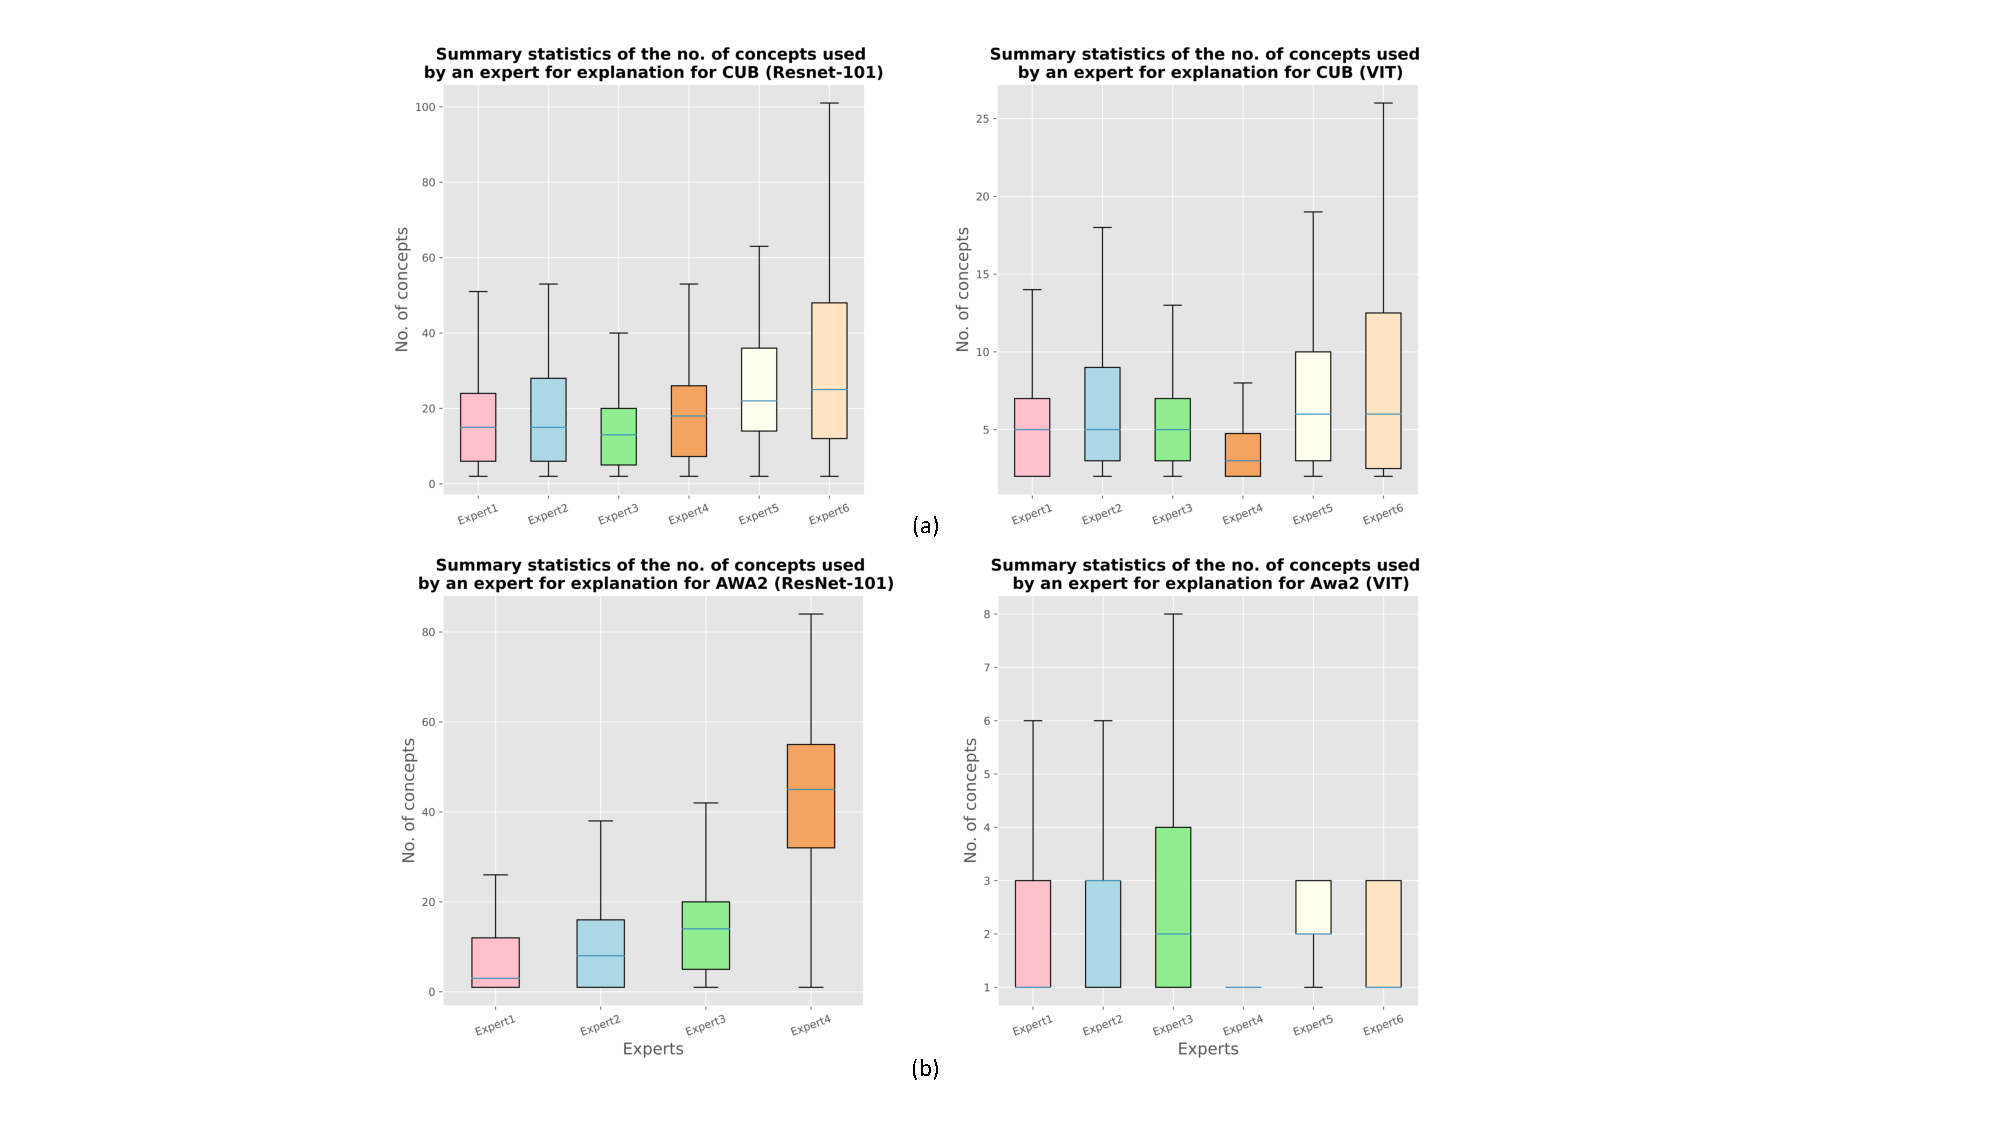
\includegraphics[width=1\textwidth]{figures/Supp/Summary_stats_vit_resnet.pdf}
\caption{Summary statistics of the number of concepts utilized by various experts of datasets (a) CUB -200(top row) and (b) Awa2 (bottom row). In general, we can see that experts carving out the explanations from VIT often uses less number of concepts.}
\label{fig:stats_ex_cub}
\end{figure}



\cref{fig:stats_ex_cub} shows the summary statistics for multiclass classification vision datasets. For both datasets, we observe that the VIT-based MoIE uses fewer concepts for explanation than their ResNet-based counterparts. For example, for the CUB-200 dataset, expert6 of VIT-backbone requires 25 concepts compared to 105 by expert6 of ResNet-101-backbone (~\cref{fig:stats_ex_cub}a). The 105 concepts by expert6 is the highest number of concepts utilized by any expert for CUB-200. Similarly, for Awa2, the highest number concept used by an expert is 8 for the VIT-based backbone compared to 80 for the ResNet-101-based backbone (\cref{fig:stats_ex_cub}b).
As mentioned before, the average number of concepts for class $j$ = $\frac{\sum\text{all concepts for the samples belong to class $j$}}{\text{\# samples of class $j$}}$. We can see that for ResNet-101, on average 80 concepts are required to explain a sample correctly for the class ``Rhinoceros\_Auklet'' (expert3 in~\cref{fig:cnn_cub_concept_3_4} a). However, for VIT, only 6 concepts are needed to explain a sample correctly ``Rhinoceros\_Auklet'' (expert3  in~\cref{fig:vit_cub_concept_3_4} a). From both of these figures, we can see that different experts require a different number of concepts to explain the same class. For example,~\cref{fig:vit_cub_concept_1_2}  (b) and~\cref{fig:vit_cub_concept_5_6} (b) reveal that experts 2 and 6 require 25 and 58 concepts on average to explain ``Artic\_Tern'' correctly respectively for VIT-derived MoIE.


% Figures \ref{fig:vit_cub_concept_1_2}, \ref{fig:vit_cub_concept_3_4} and \ref{fig:vit_cub_concept_5_6} display the average number of concepts required to predict a bird species correctly in the Cub-200 dataset for all the experts of VIT as backbones. Also, Figures \ref{fig:cnn_cub_concept_1_2}, \ref{fig:cnn_cub_concept_3_4} and \ref{fig:cnn_cub_concept_5_6} display the same for the ResNet-101 based counterparts. 
~\cref{fig:Awa2_VIT_a}, ~\cref{fig:Awa2_VIT_b},~\cref{fig:Awa2_VIT_c} display the average number of concepts required to predict an animal species correctly in the Awa2 dataset for VIT as backbones. Similarly~\cref{fig:Awa2_CNN_a} and~\cref{fig:Awa2_CNN_b} display the average number of concepts required to predict an animal species correctly in the Awa2 dataset for ResNet101 as backbones. We can see that for ResNet101, on average, 80 concepts are required to explain a sample correctly for the class ``Weasel'' (Expert1 in~\cref{fig:Awa2_CNN_a} a). However, for VIT, only three concepts are needed to explain a sample correctly for ``Weasel'' (Expert 6 in~\cref{fig:Awa2_VIT_c} f). Also, from both of these figures, we can see that different experts require different number concepts to explain the same class. For example,~\cref {fig:Awa2_VIT_c} (e) and (f) reveal that experts 5 and 6 require 4 and 30 concepts on average to explain ``Wolf'' correctly.

\begin{figure}
\centering
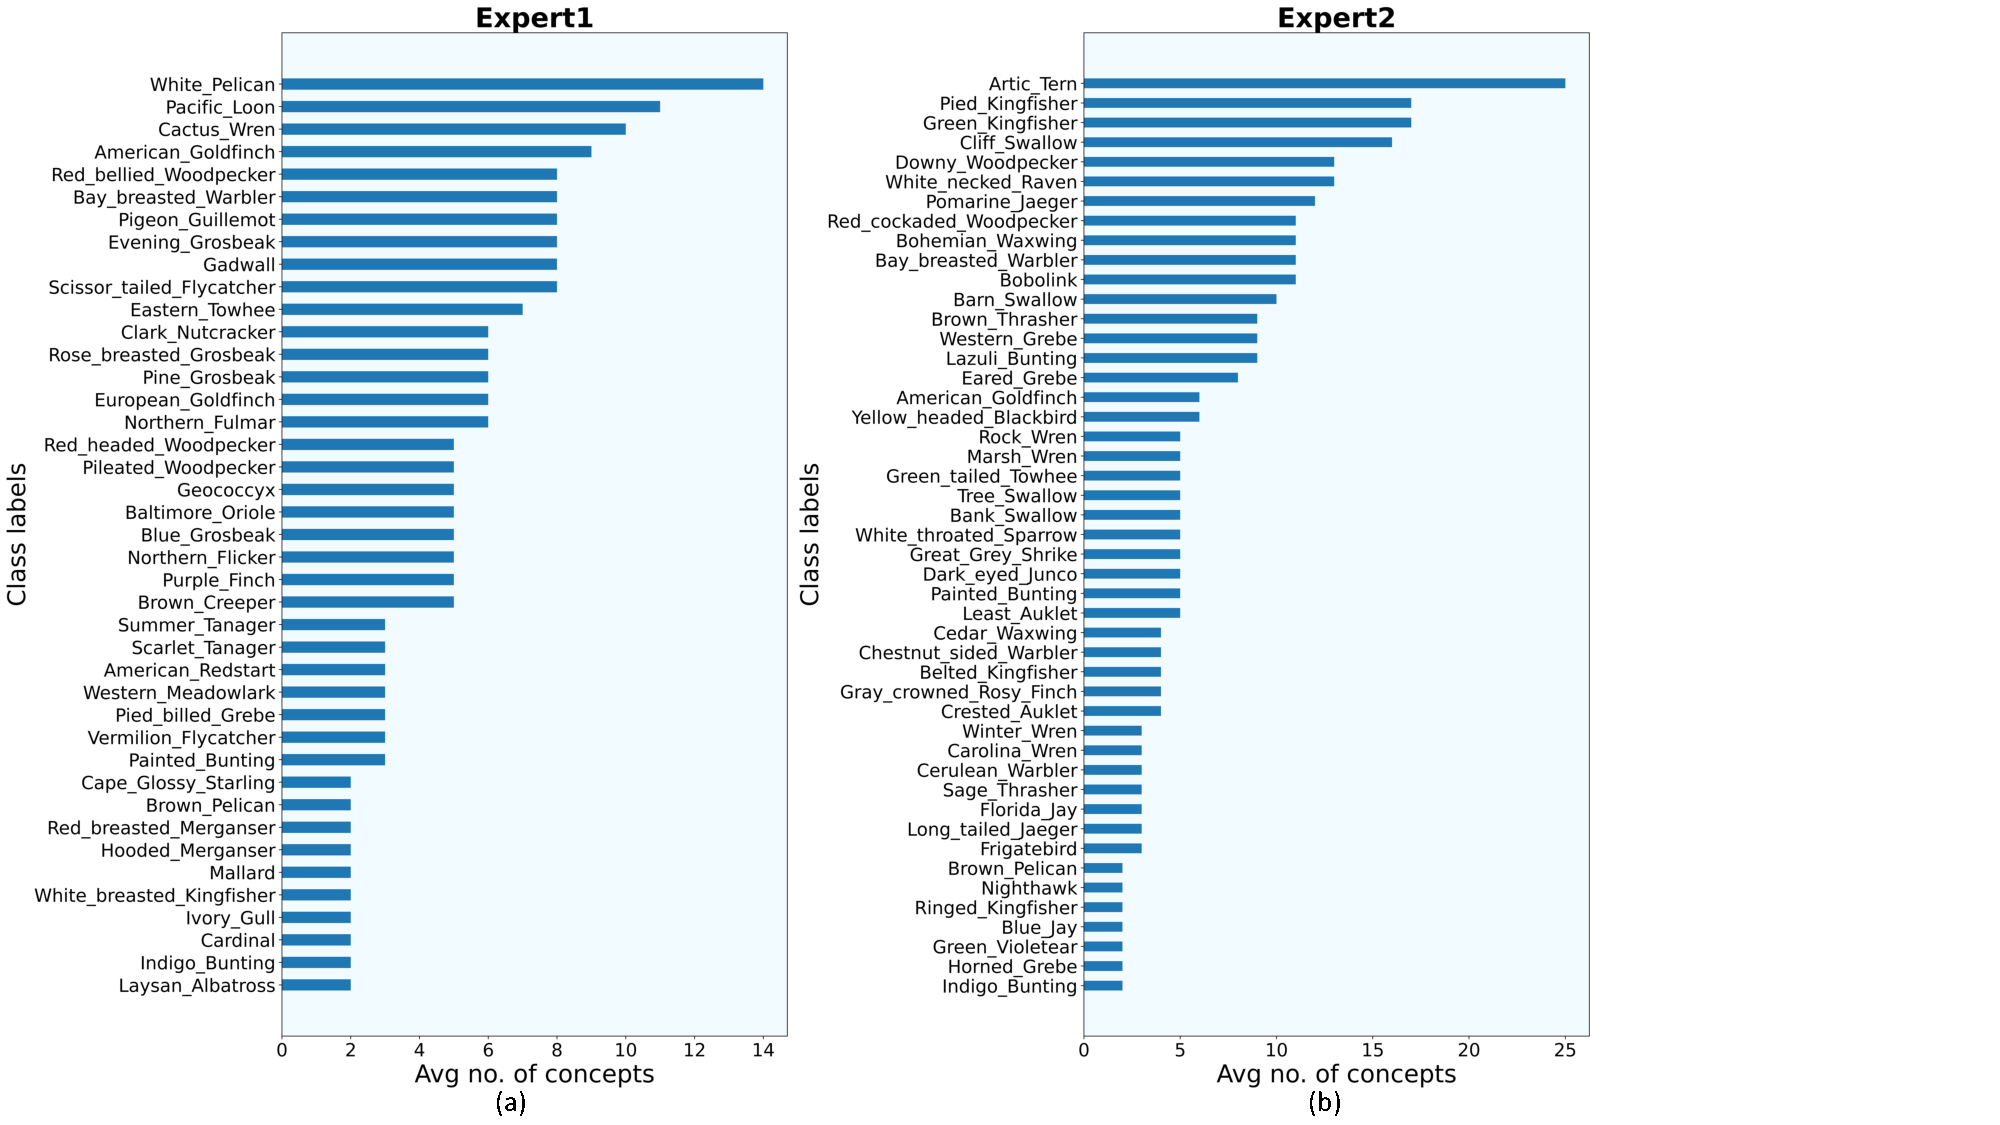
\includegraphics[width=14cm, height=13cm]
{figures/Supp/Avg_concept_class_VIT_cub_1.pdf}
\caption{Class labels (Bird species) vs. avg concepts using VIT as the backbone for CUB-200 by (a) Expert1 (b) Expert2. Each bar in this plot indicates the average number of concepts required to explain each sample of that bird species correctly. For example according to (a) expert1 requires 14 concepts to explain an instance of ``White Pelican''.}
\label{fig:vit_cub_concept_1_2}
\end{figure}

\begin{figure}
\centering
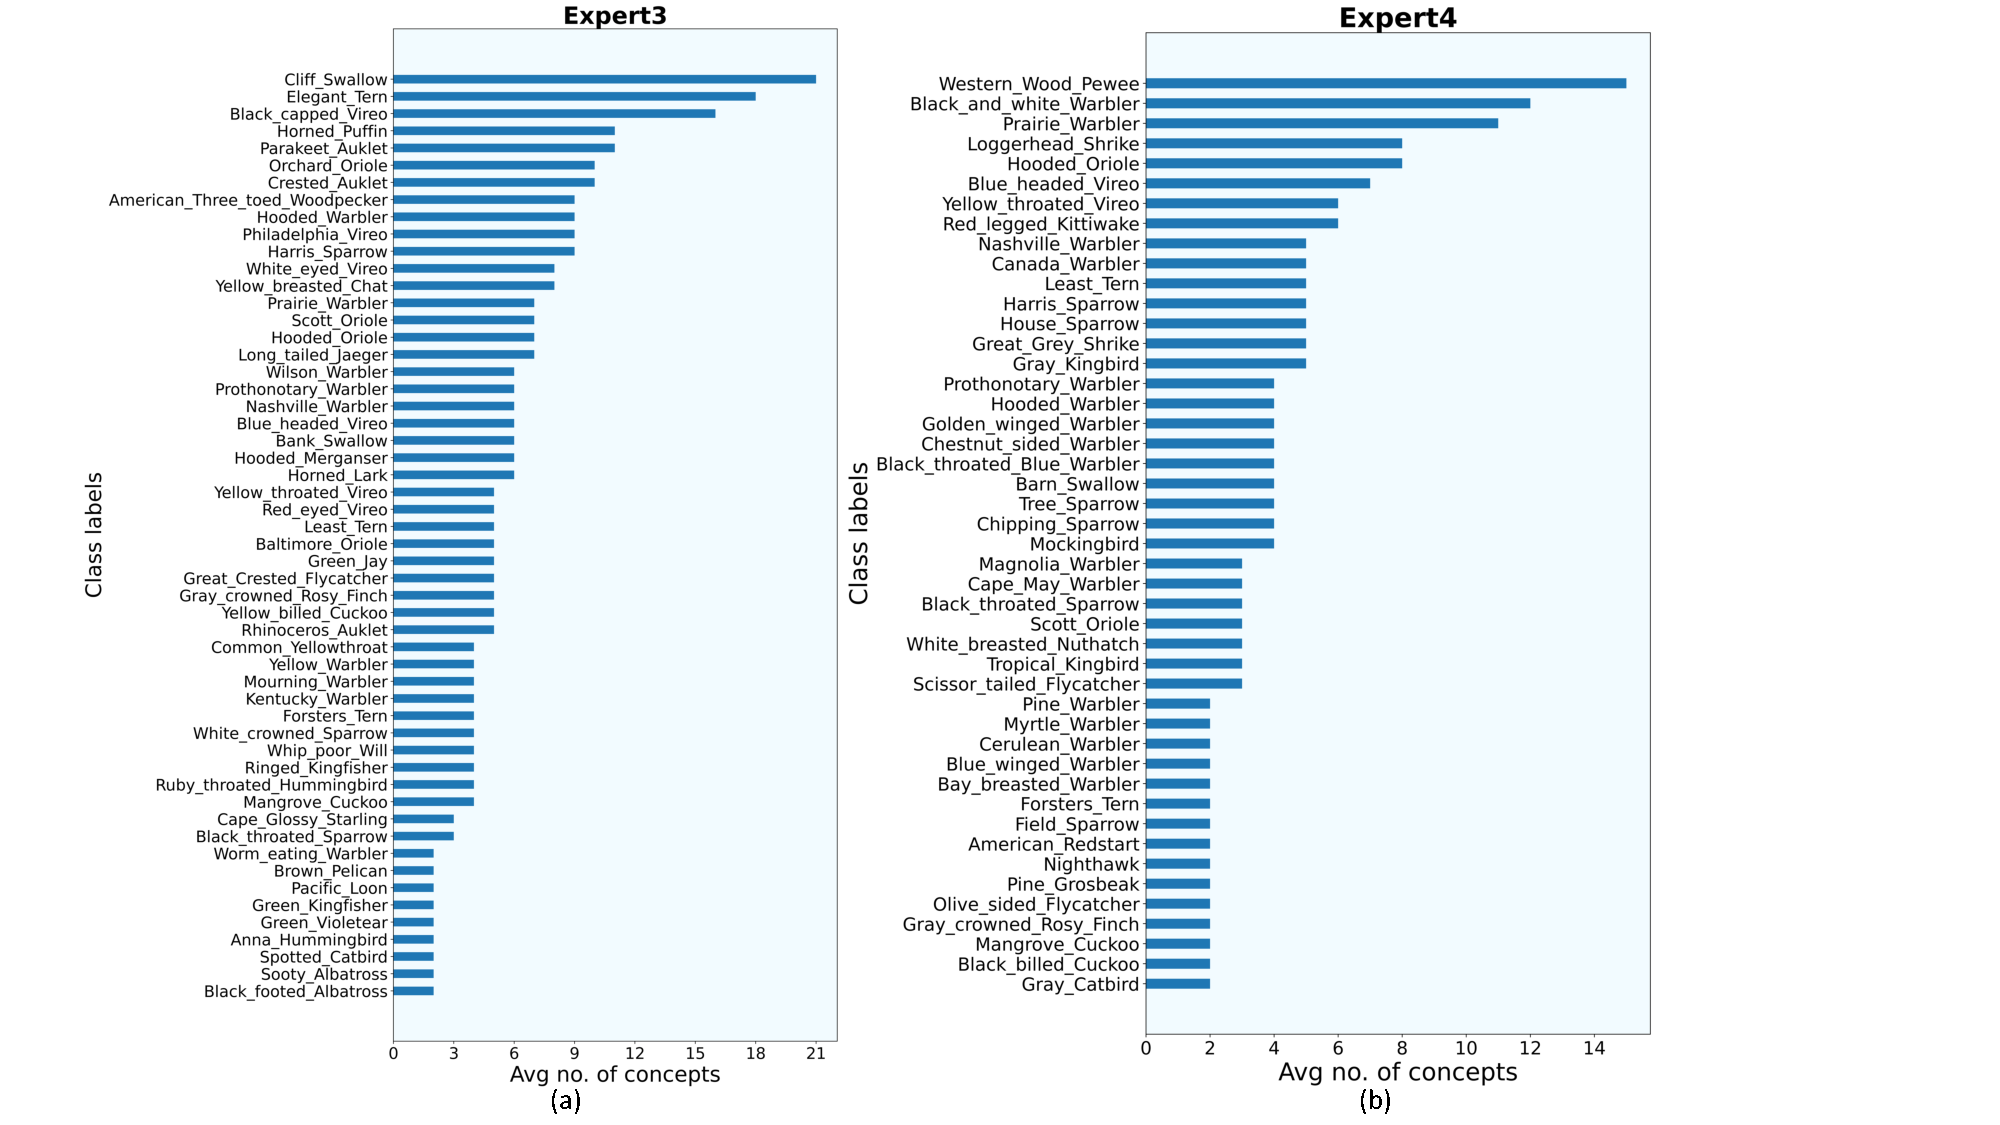
\includegraphics[width=14cm, height=13cm]
{figures/Supp/Avg_concept_class_VIT_cub_2.pdf}
\caption{Class labels (Bird species) vs. avg concepts using VIT as the backbone for CUB-200 by (a) Expert3 (b) Expert4. Each bar in this plot indicates the average number of concepts required to explain each sample of that bird species correctly. For example according to (a) expert3 requires 21 concepts to explain an instance of ``Cliff Swallow''.}
\label{fig:vit_cub_concept_3_4}
\end{figure}

\begin{figure}
\centering
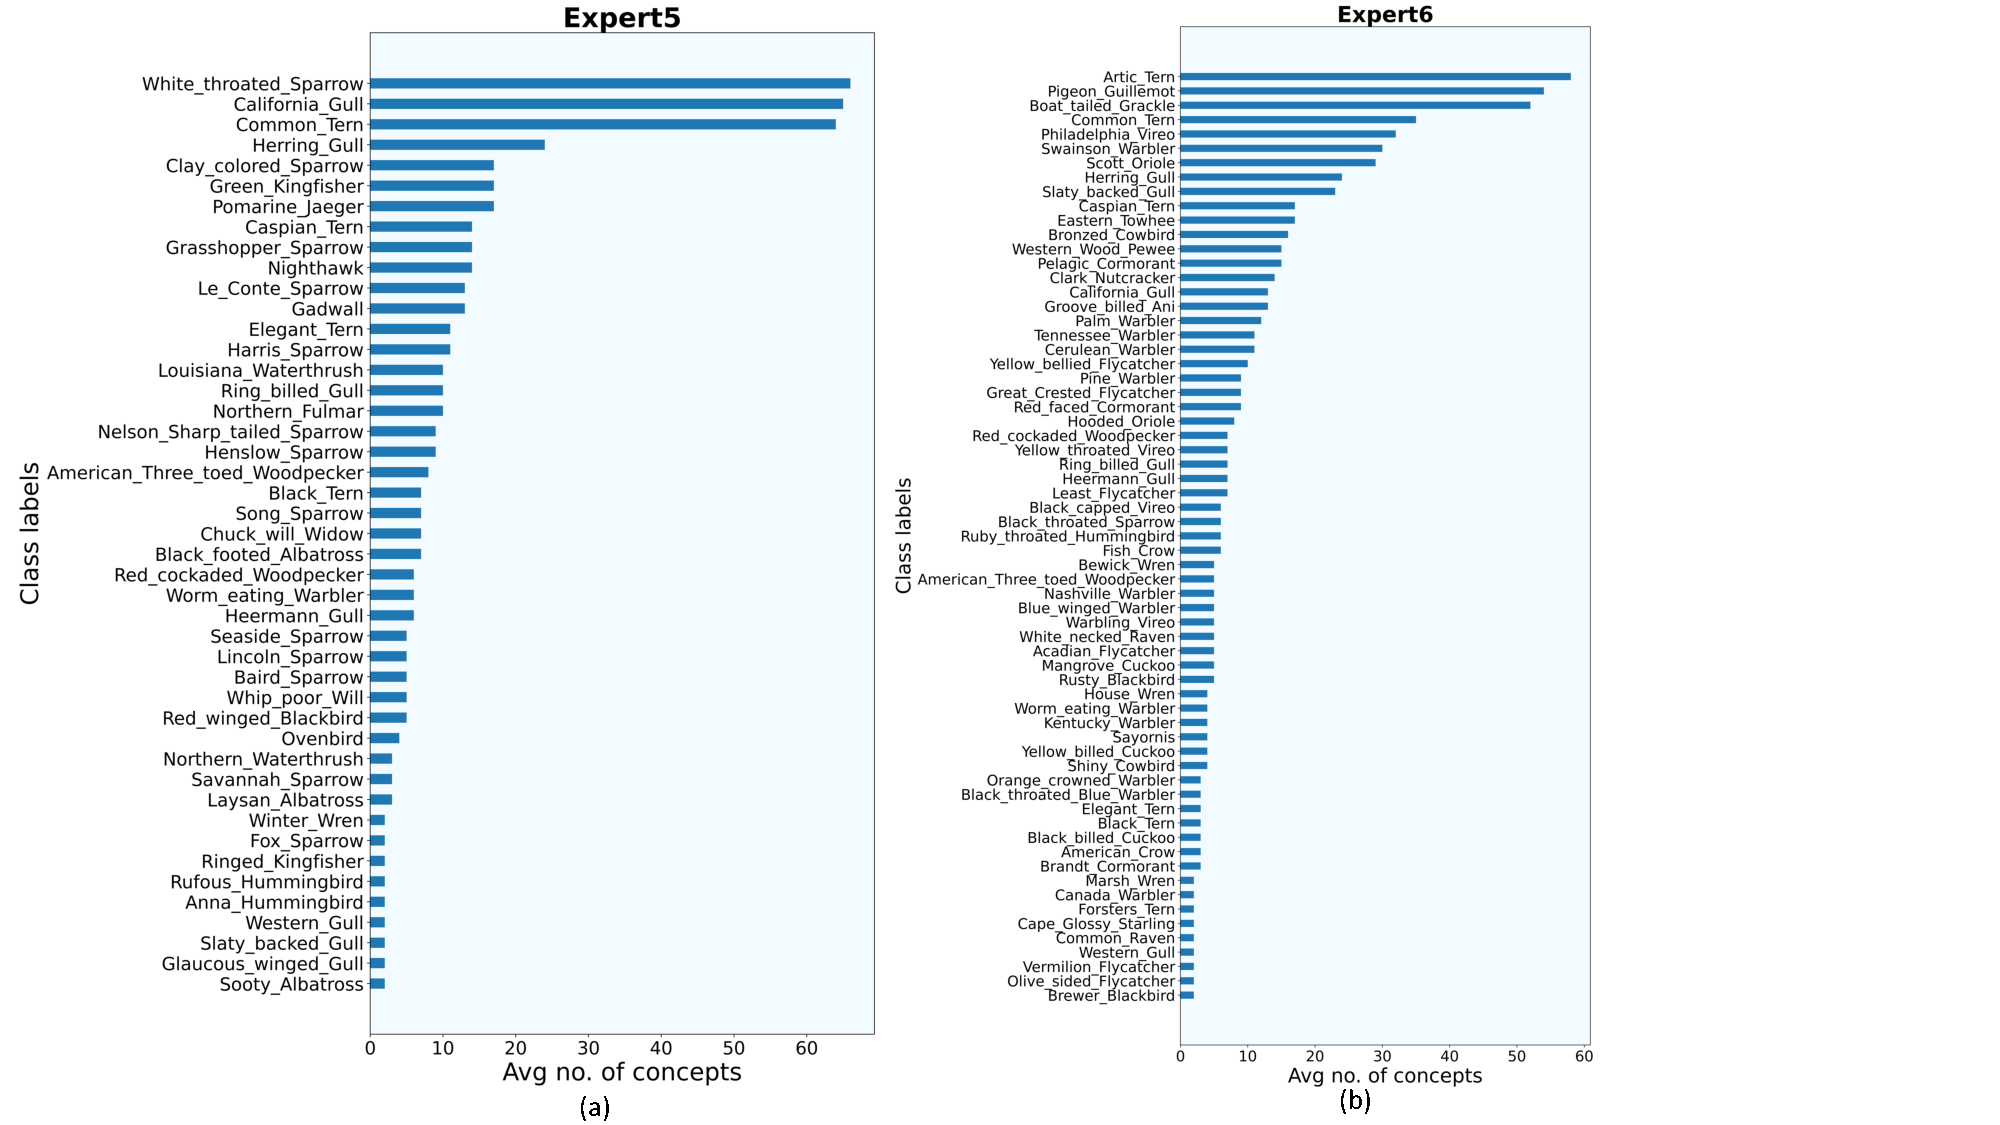
\includegraphics[width=14cm, height=13cm]
{figures/Supp/Avg_concept_class_VIT_cub_3.pdf}
\caption{Class labels (Bird species) vs. avg concepts using VIT as the backbone for CUB-200 by (a) Expert5 (b) Expert6. Each bar in this plot indicates the average number of concepts required to explain each sample of that bird species correctly. For example according to (a) expert5 requires approximately 65 concepts to explain an instance of ``White throated sparrow''.}
\label{fig:vit_cub_concept_5_6}
\end{figure}

% CNN
\begin{figure}
\centering
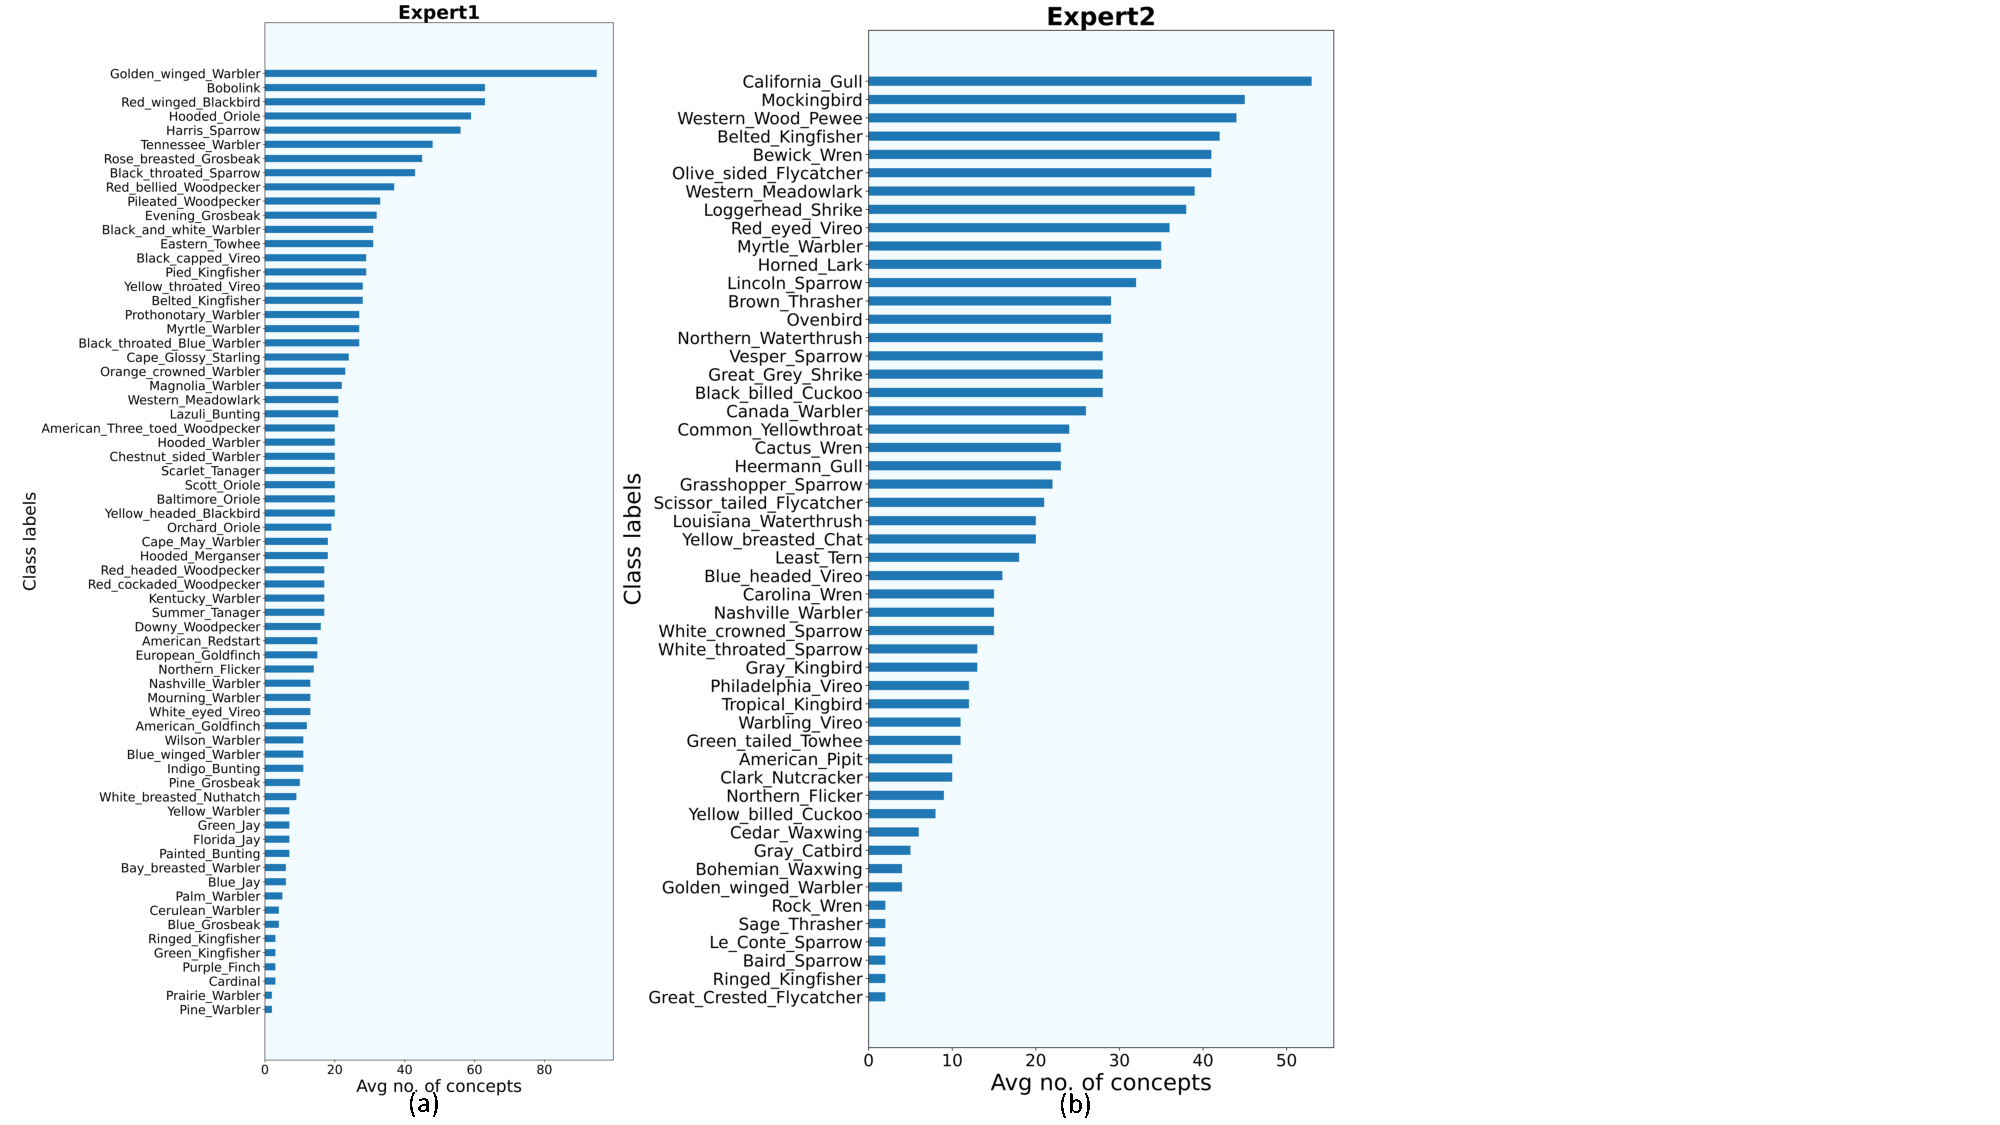
\includegraphics[width=15cm, height=13cm]
{figures/Supp/Avg_concept_class_CNN_cub_1.pdf}
\caption{Class labels (Bird species) vs. avg concepts using ResNet-101 as the backbone for CUB-200 by (a) Expert1 (b) Expert2. Each bar in this plot indicates the average number of concepts required to explain each sample of that bird species correctly. For example according to (a) expert1 requires approximately 85 concepts to explain an instance of ``Golden winged warbler''.}
\label{fig:cnn_cub_concept_1_2}
\end{figure}

\begin{figure}
\centering
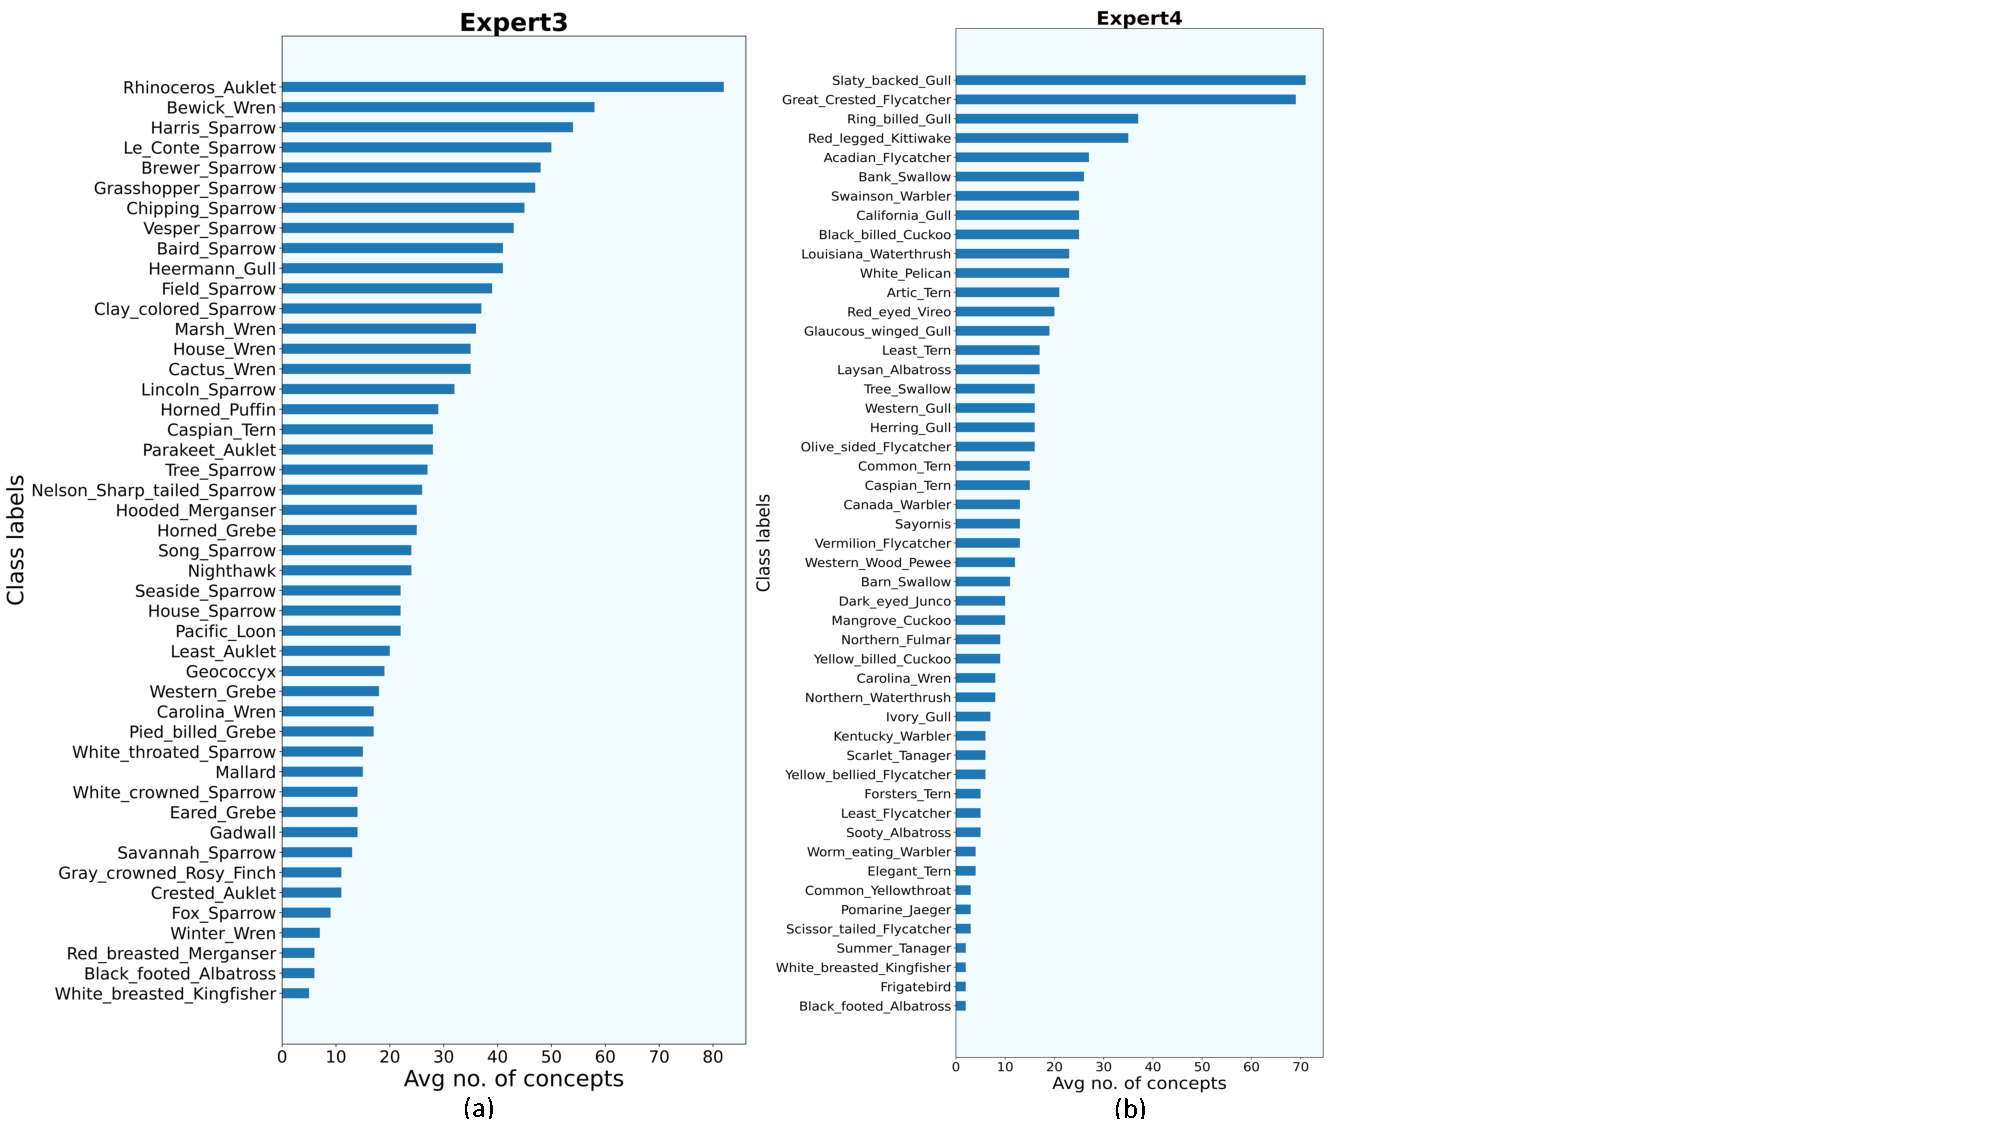
\includegraphics[width=15cm, height=13cm]
{figures/Supp/Avg_concept_class_CNN_cub_2.pdf}
\caption{Class labels (Bird species) vs. avg concepts using  ResNet-101 as the backbone for CUB-200 by (a) Expert3 (b) Expert4. Each bar in this plot indicates the average number of concepts required to explain each sample of that bird species correctly. For example according to (a) expert3 requires approximately 82 concepts to explain an instance of ``Rhinoceros auklet''.}
\label{fig:cnn_cub_concept_3_4}
\end{figure}

\begin{figure}
\centering
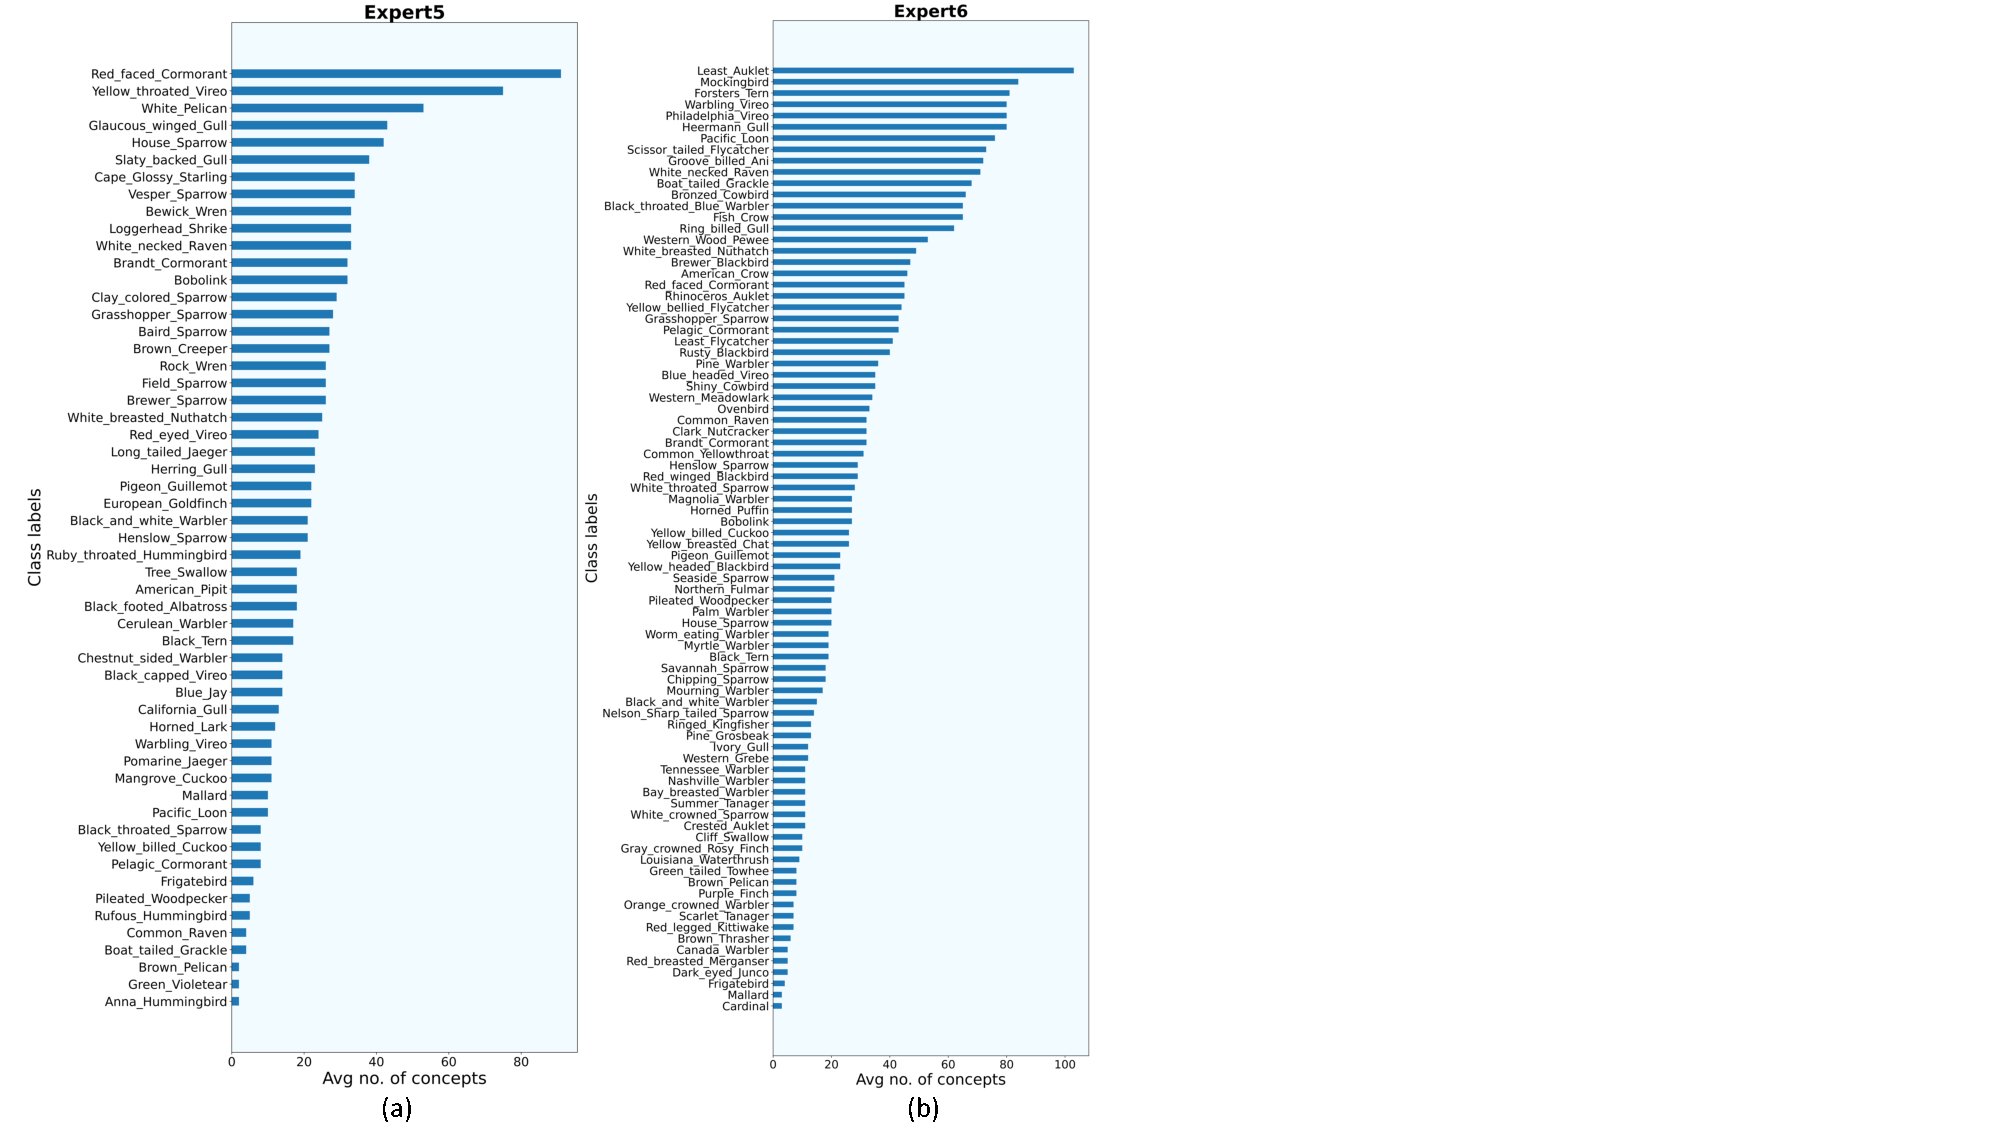
\includegraphics[width=1\linewidth]
{figures/Supp/Avg_concept_class_CNN_cub_3.pdf}
\caption{Class labels (Bird species) vs. avg concepts using  ResNet-101 as the backbone for CUB-200 by (a) Expert5 (b) Expert6. Each bar in this plot indicates the average number of concepts required to explain each sample of that bird species correctly. For example according to (a) expert5 requires approximately 85 concepts to explain an instance of ``Red faced carmorant''.}
\label{fig:cnn_cub_concept_5_6}
\end{figure}

\begin{figure}
\centering
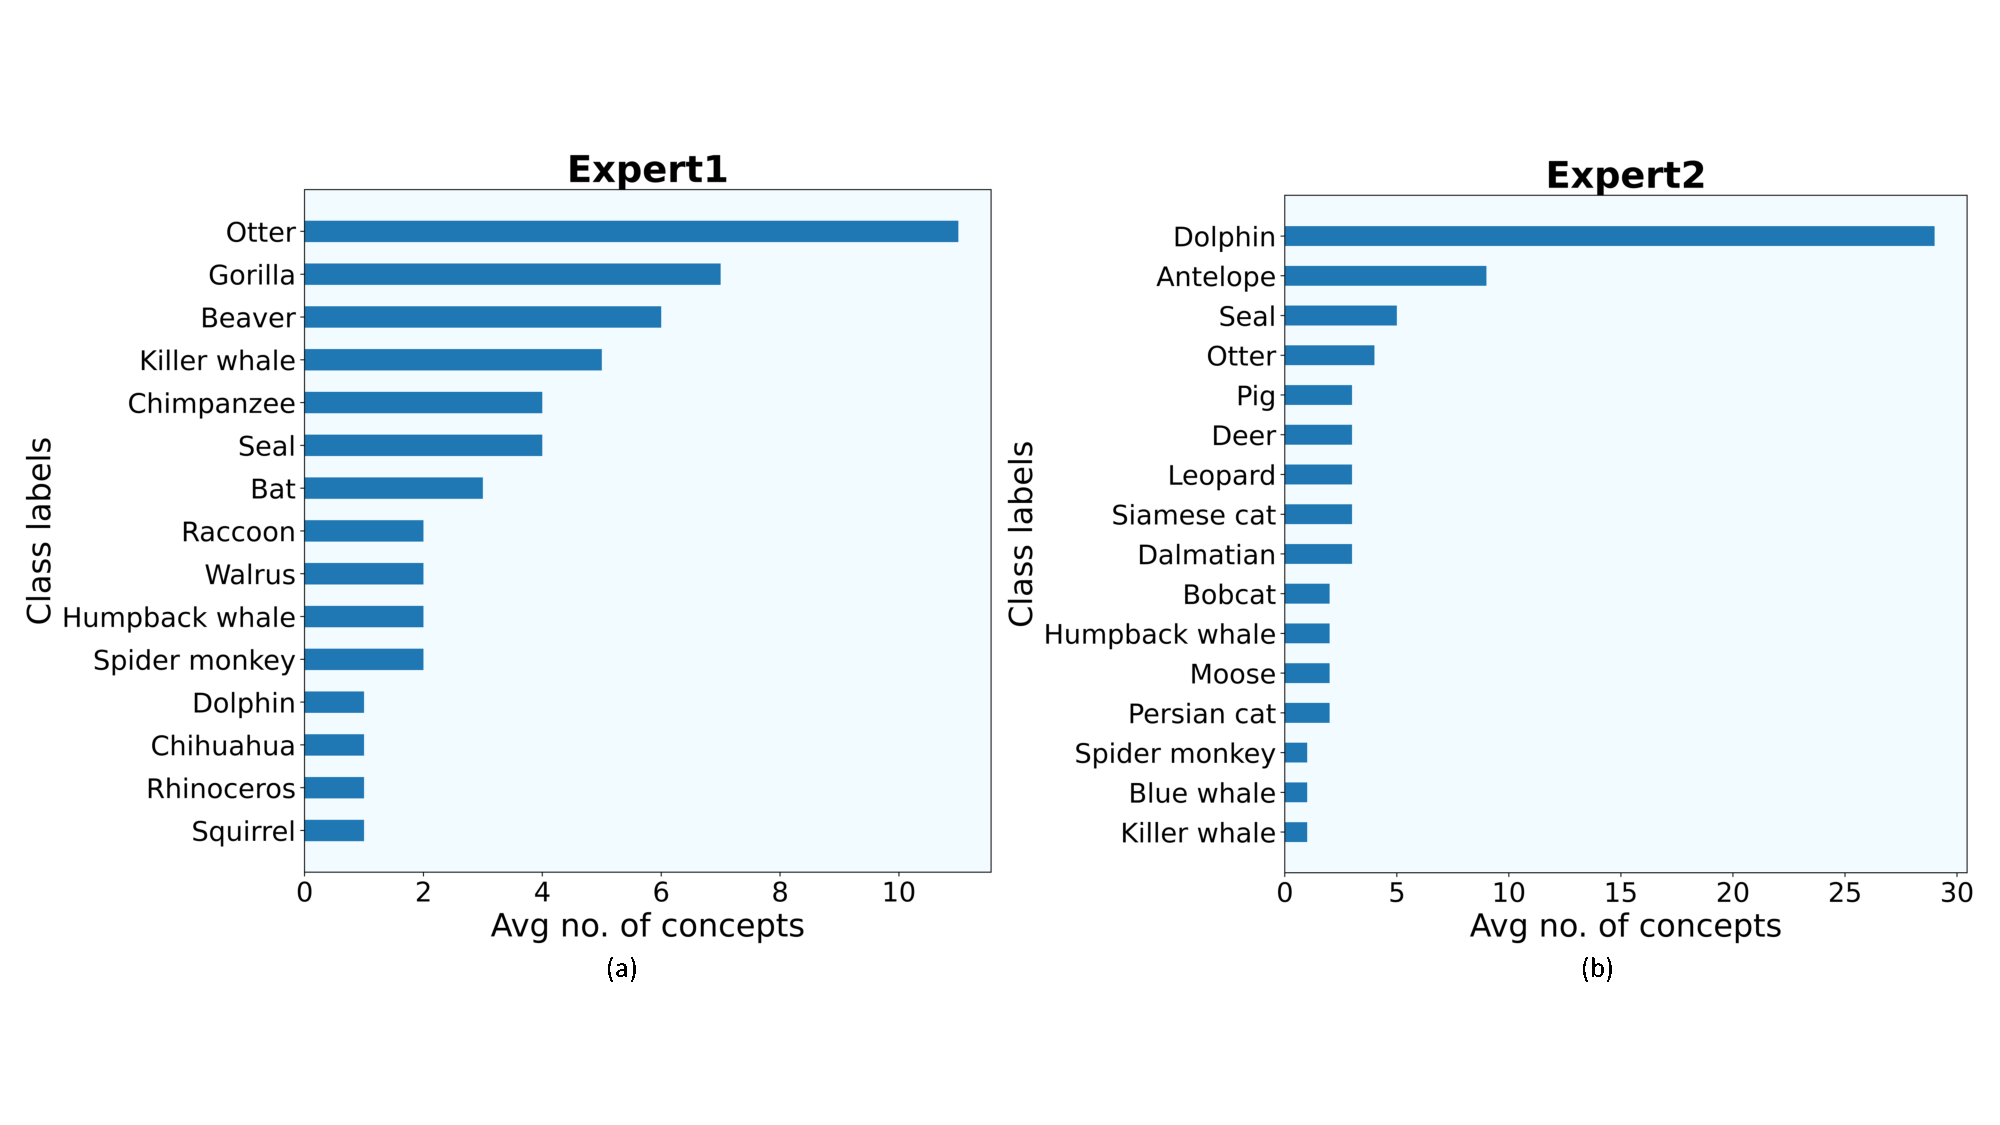
\includegraphics[width=1\linewidth]
{figures/Supp/Avg_concept_class_VIT_Awa2_1.pdf}
\caption{Class labels (Animal species) vs. avg concepts using VIT as the backbone for Awa2. Each bar in this plot indicates the average number of concepts required to explain each sample of that animal species correctly. For example according to (c) expert1 requires approximately 12 concepts to explain an instance of ``Otter''.}
\label{fig:Awa2_VIT_a}
\end{figure}

\begin{figure}
\centering
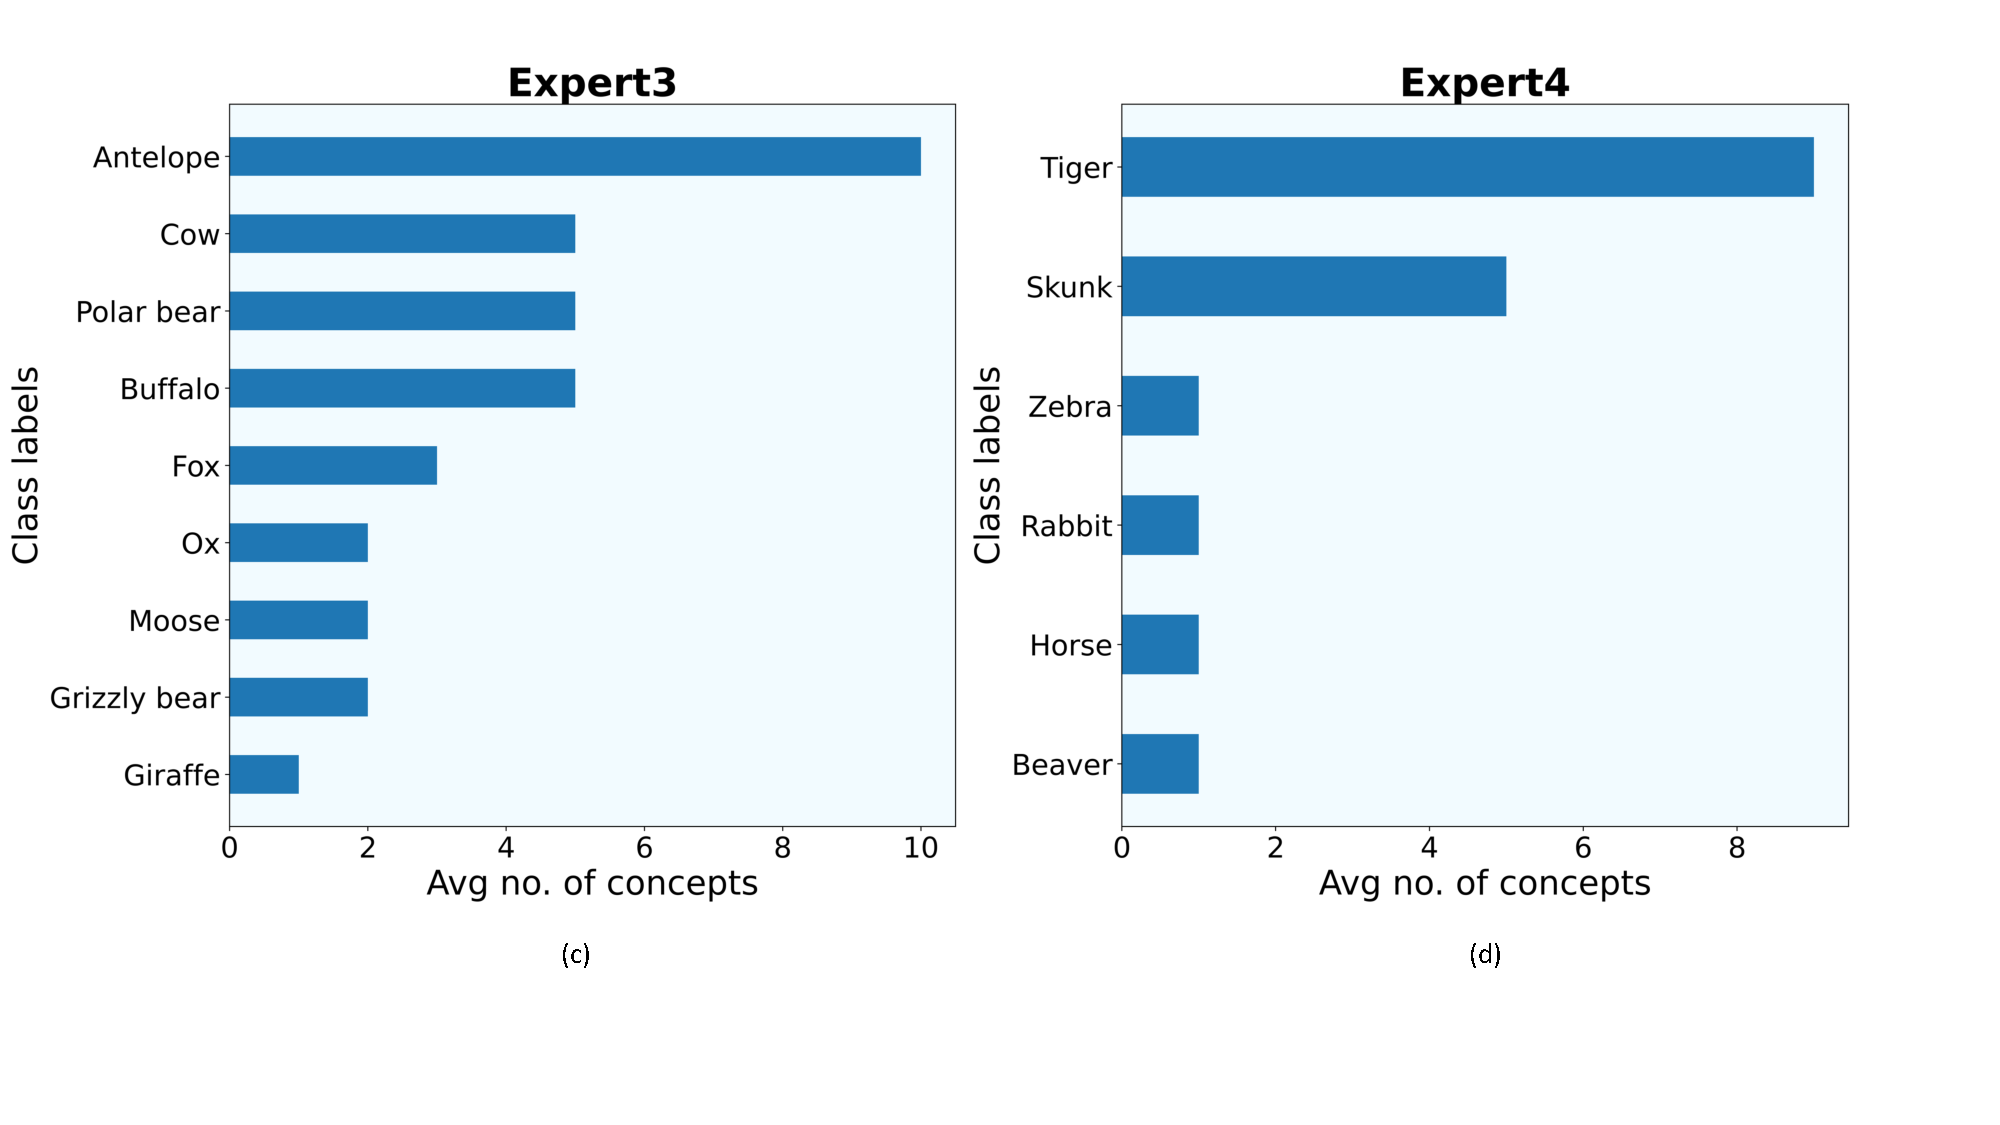
\includegraphics[width=1\linewidth]
{figures/Supp/Avg_concept_class_VIT_Awa2_2.pdf}
\caption{Class labels (Animal species) vs. avg concepts using VIT as the backbone for Awa2. Each bar in this plot indicates the average number of concepts required to explain each sample of that animal species correctly. For example according to (c) expert3 requires approximately 10 concepts to explain an instance of ``Antelope''.}
\label{fig:Awa2_VIT_b}
\end{figure}

\begin{figure}
\centering
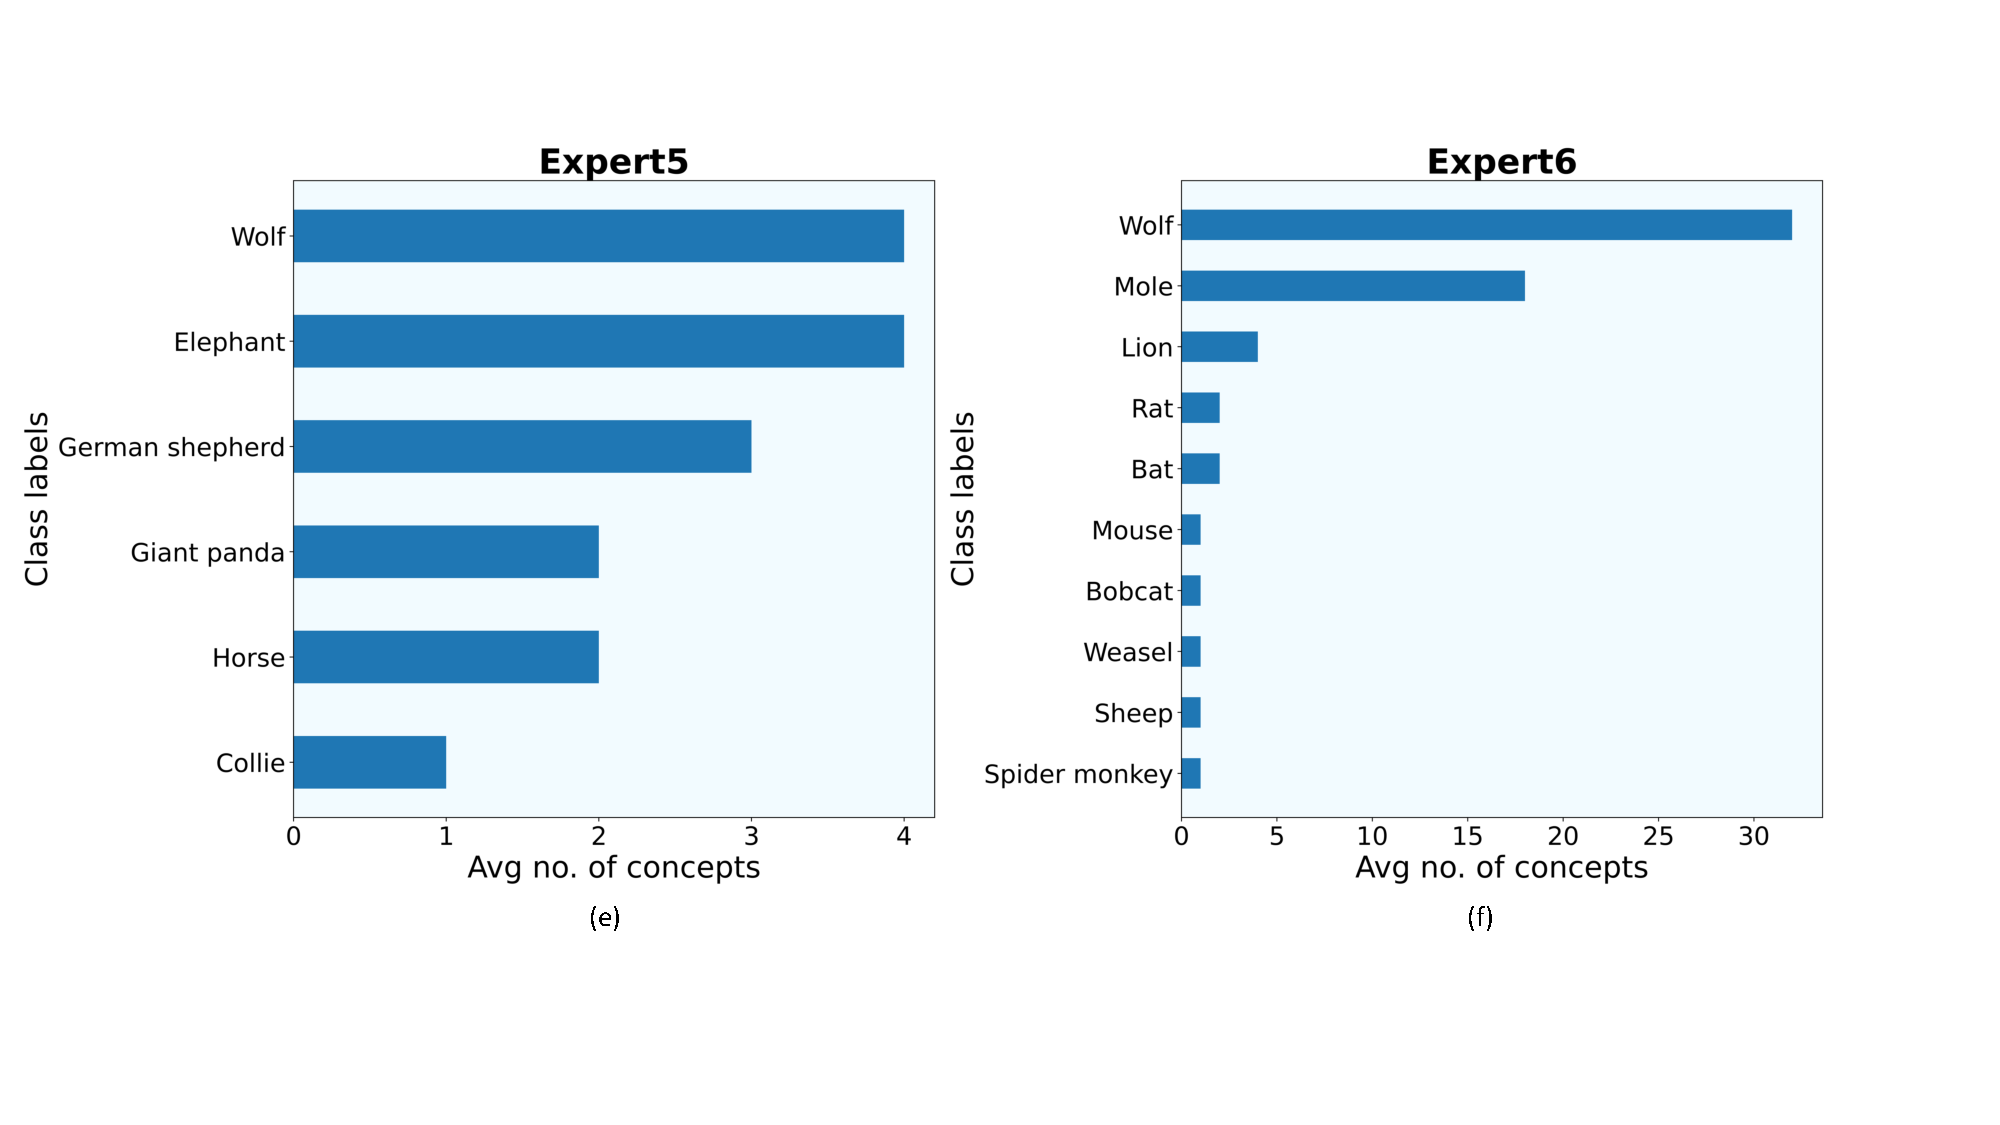
\includegraphics[width=1\linewidth]
{figures/Supp/Avg_concept_class_VIT_Awa2_3.pdf}
\caption{Class labels (Animal species) vs. avg concepts using VIT as the backbone for Awa2. Each bar in this plot indicates the average number of concepts required to explain each sample of that animal species correctly. For example according to (e) expert5 requires approximately 4 concepts to explain an instance of ``Antelope''.}
\label{fig:Awa2_VIT_c}
\end{figure}

\begin{figure}[t]
\centering
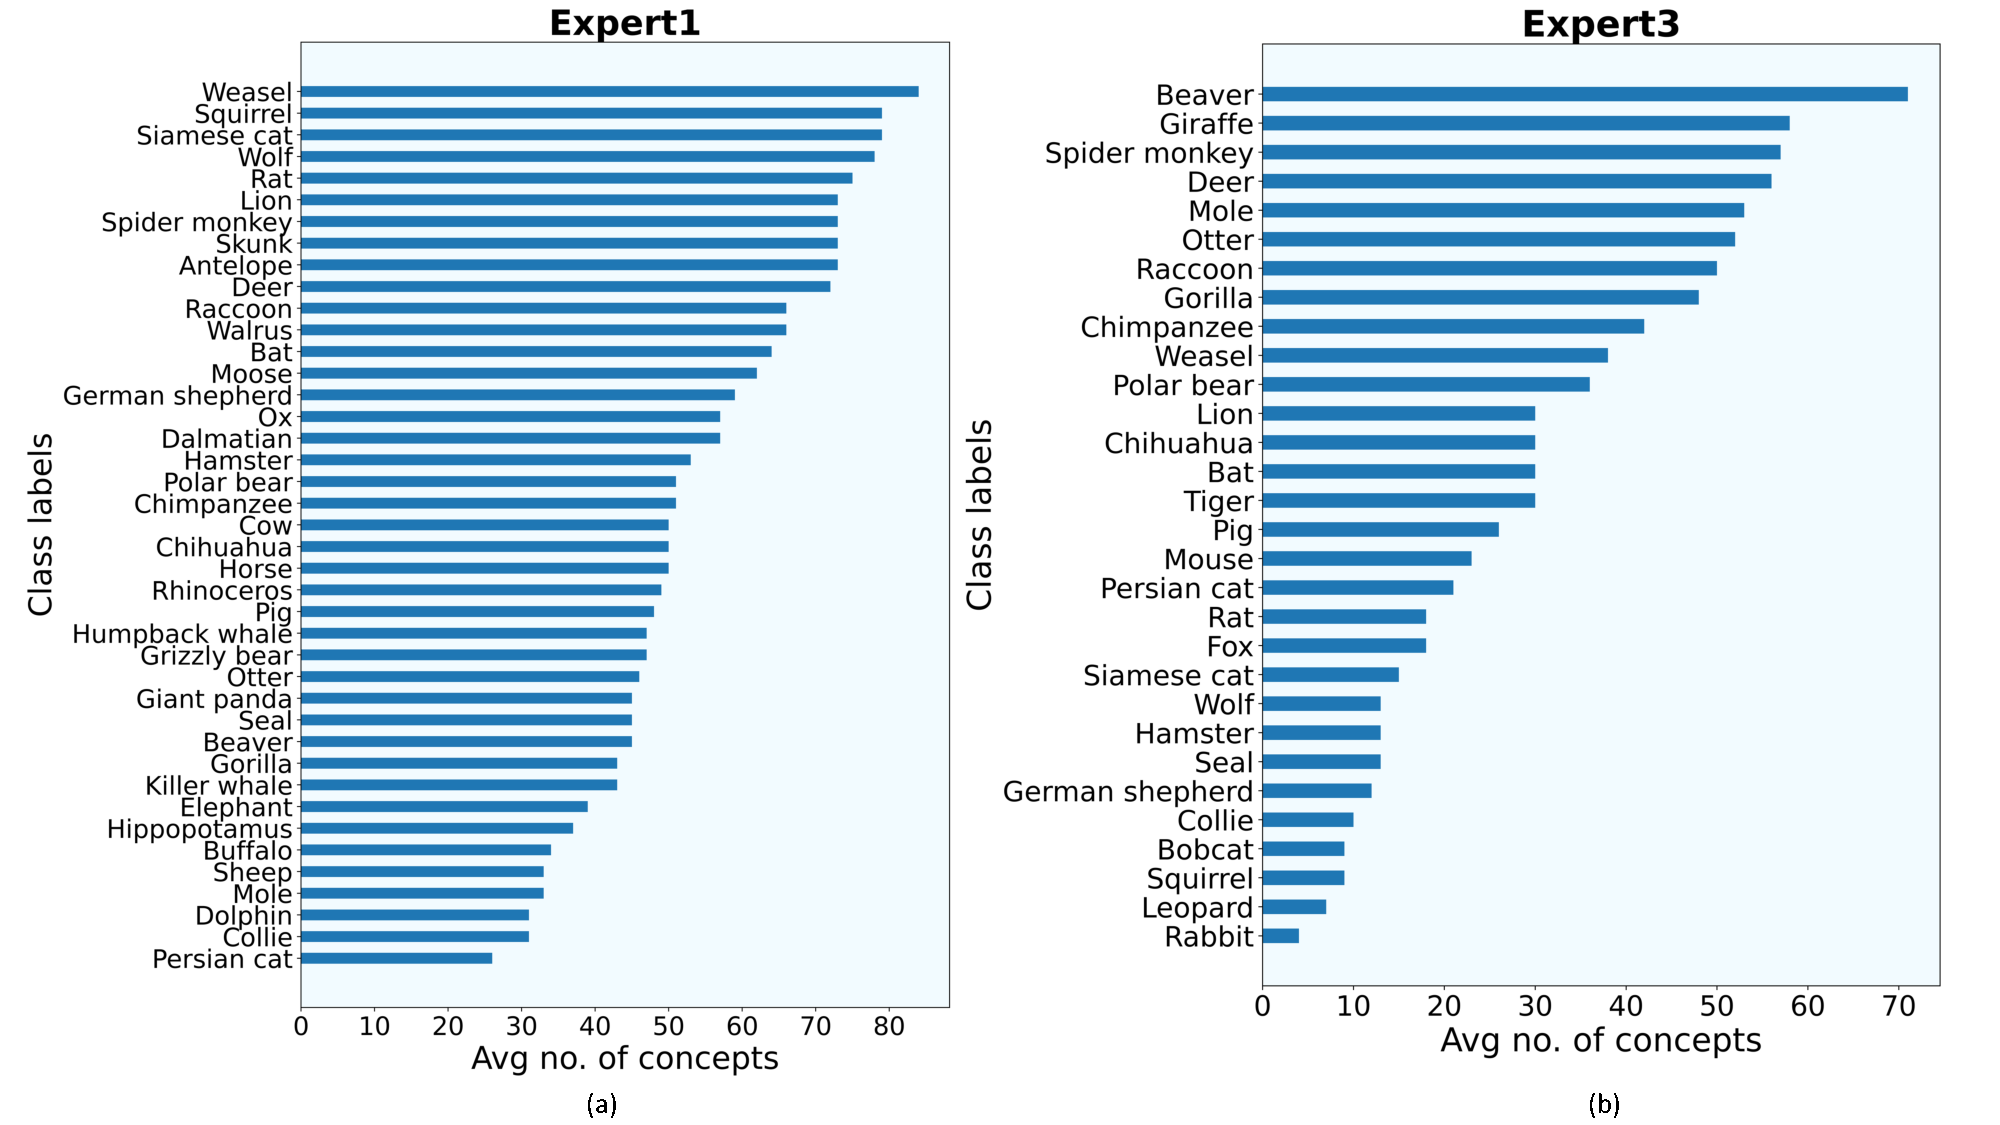
\includegraphics[width=1\linewidth]
{figures/Supp/Avg_concept_class_CNN_Awa2_1.pdf}
\caption{Class labels (Animal species) vs. avg concepts using ResNet-101 as the backbone for Awa2. Each bar in this plot indicates the average number of concepts required to explain each sample of that animal species correctly. For example according to (a) expert1 requires approximately 80 concepts to explain an instance of ``Weasel''.}
\label{fig:Awa2_CNN_a}
\end{figure}

\begin{figure}
\centering
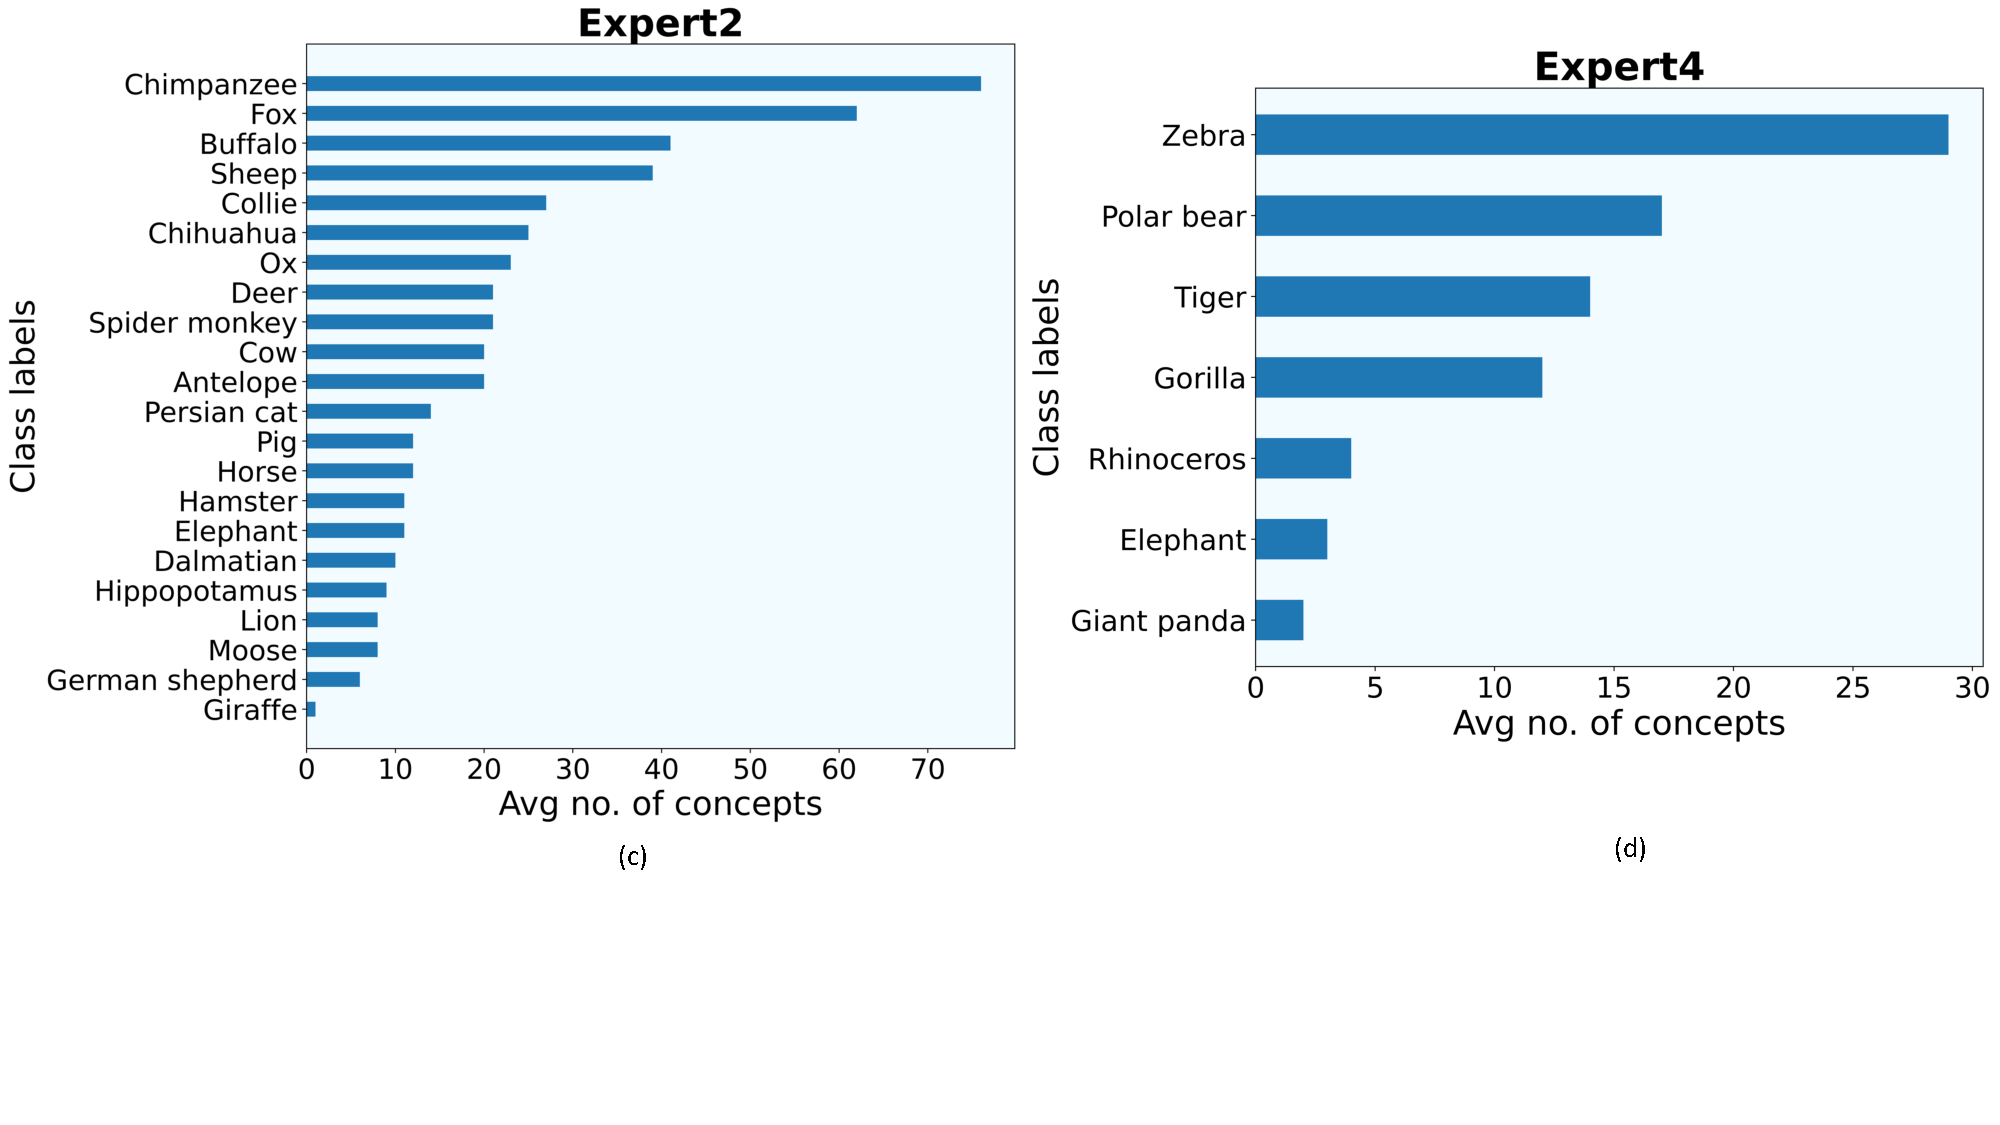
\includegraphics[width=1\linewidth]
{figures/Supp/Avg_concept_class_CNN_Awa2_2.pdf}
\caption{Class labels (Animal species) vs. avg concepts using ResNet-101 as the backbone for Awa2. Each bar in this plot indicates the average number of concepts required to explain each sample of that animal species correctly. For example according to (b) expert2 requires approximately 72 concepts to explain an instance of ``Chimpanzee''.}
\label{fig:Awa2_CNN_b}
\end{figure}



% \begin{figure}
%   \centering
%   \subfloat{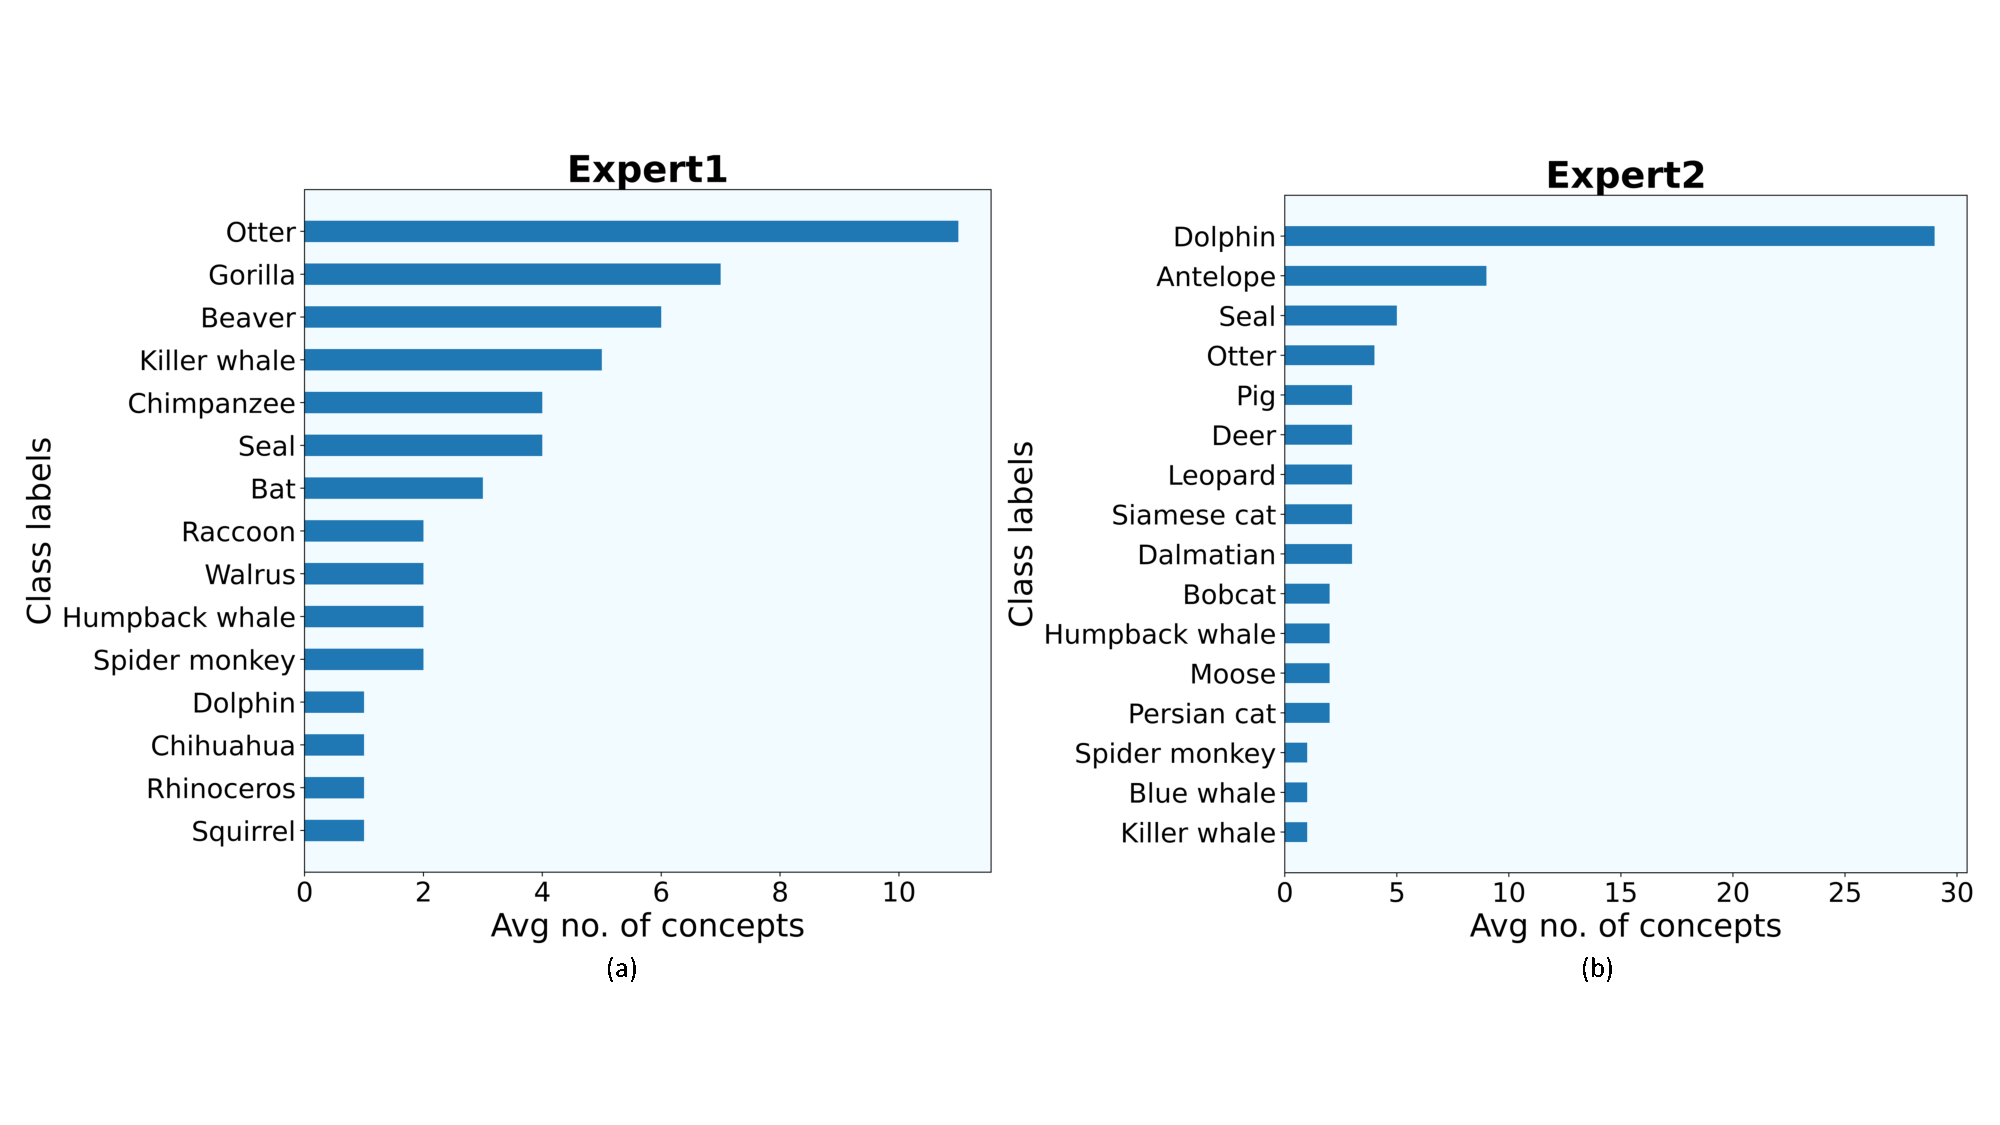
\includegraphics[width=1\textwidth]{figures/Supp/Avg_concept_class_VIT_Awa2_1.pdf} 
%   \label{fig:Awa2_VIT_a}} \\
%   \subfloat{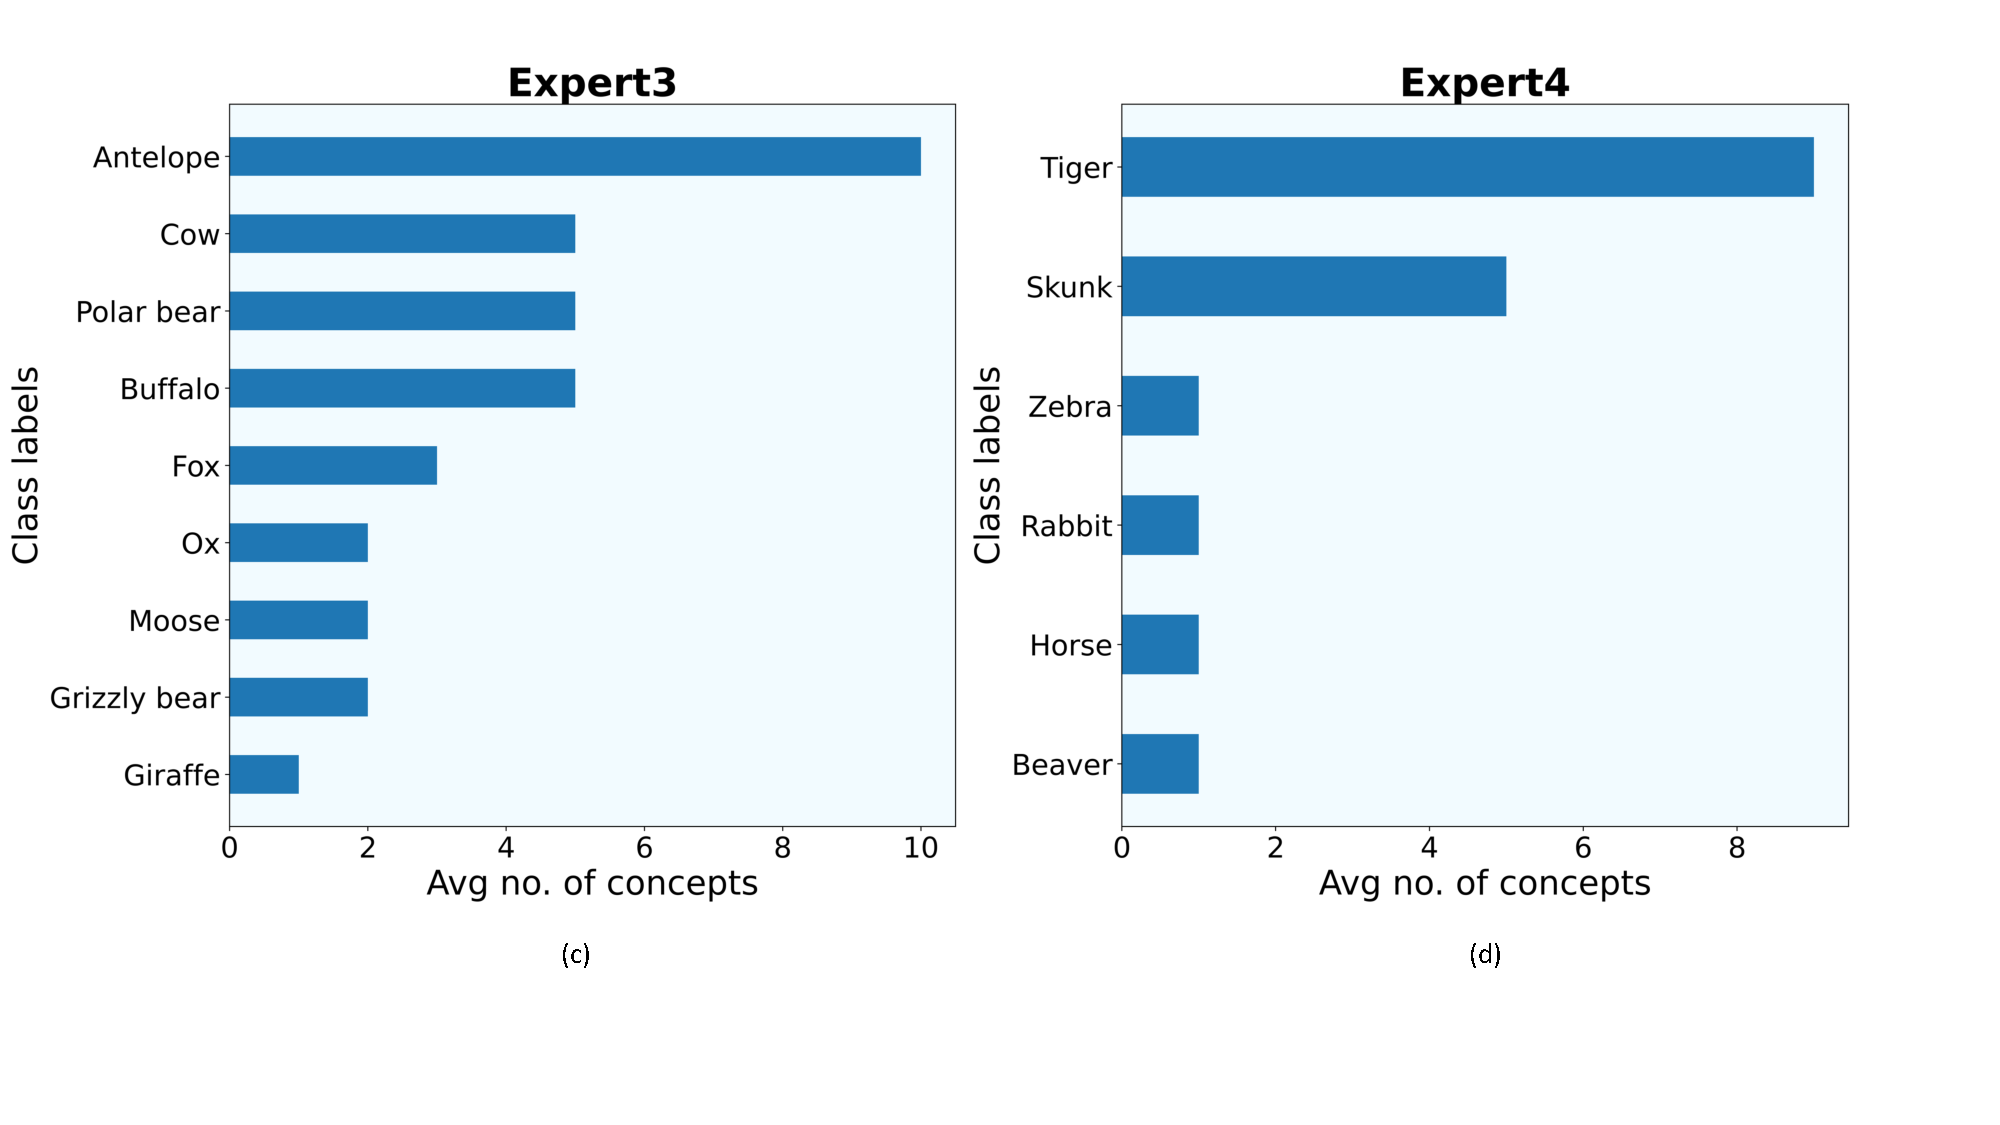
\includegraphics[width=1\textwidth]{figures/Supp/Avg_concept_class_VIT_Awa2_2.pdf} 
%   \label{fig:Awa2_VIT_b}} \\
%   \subfloat{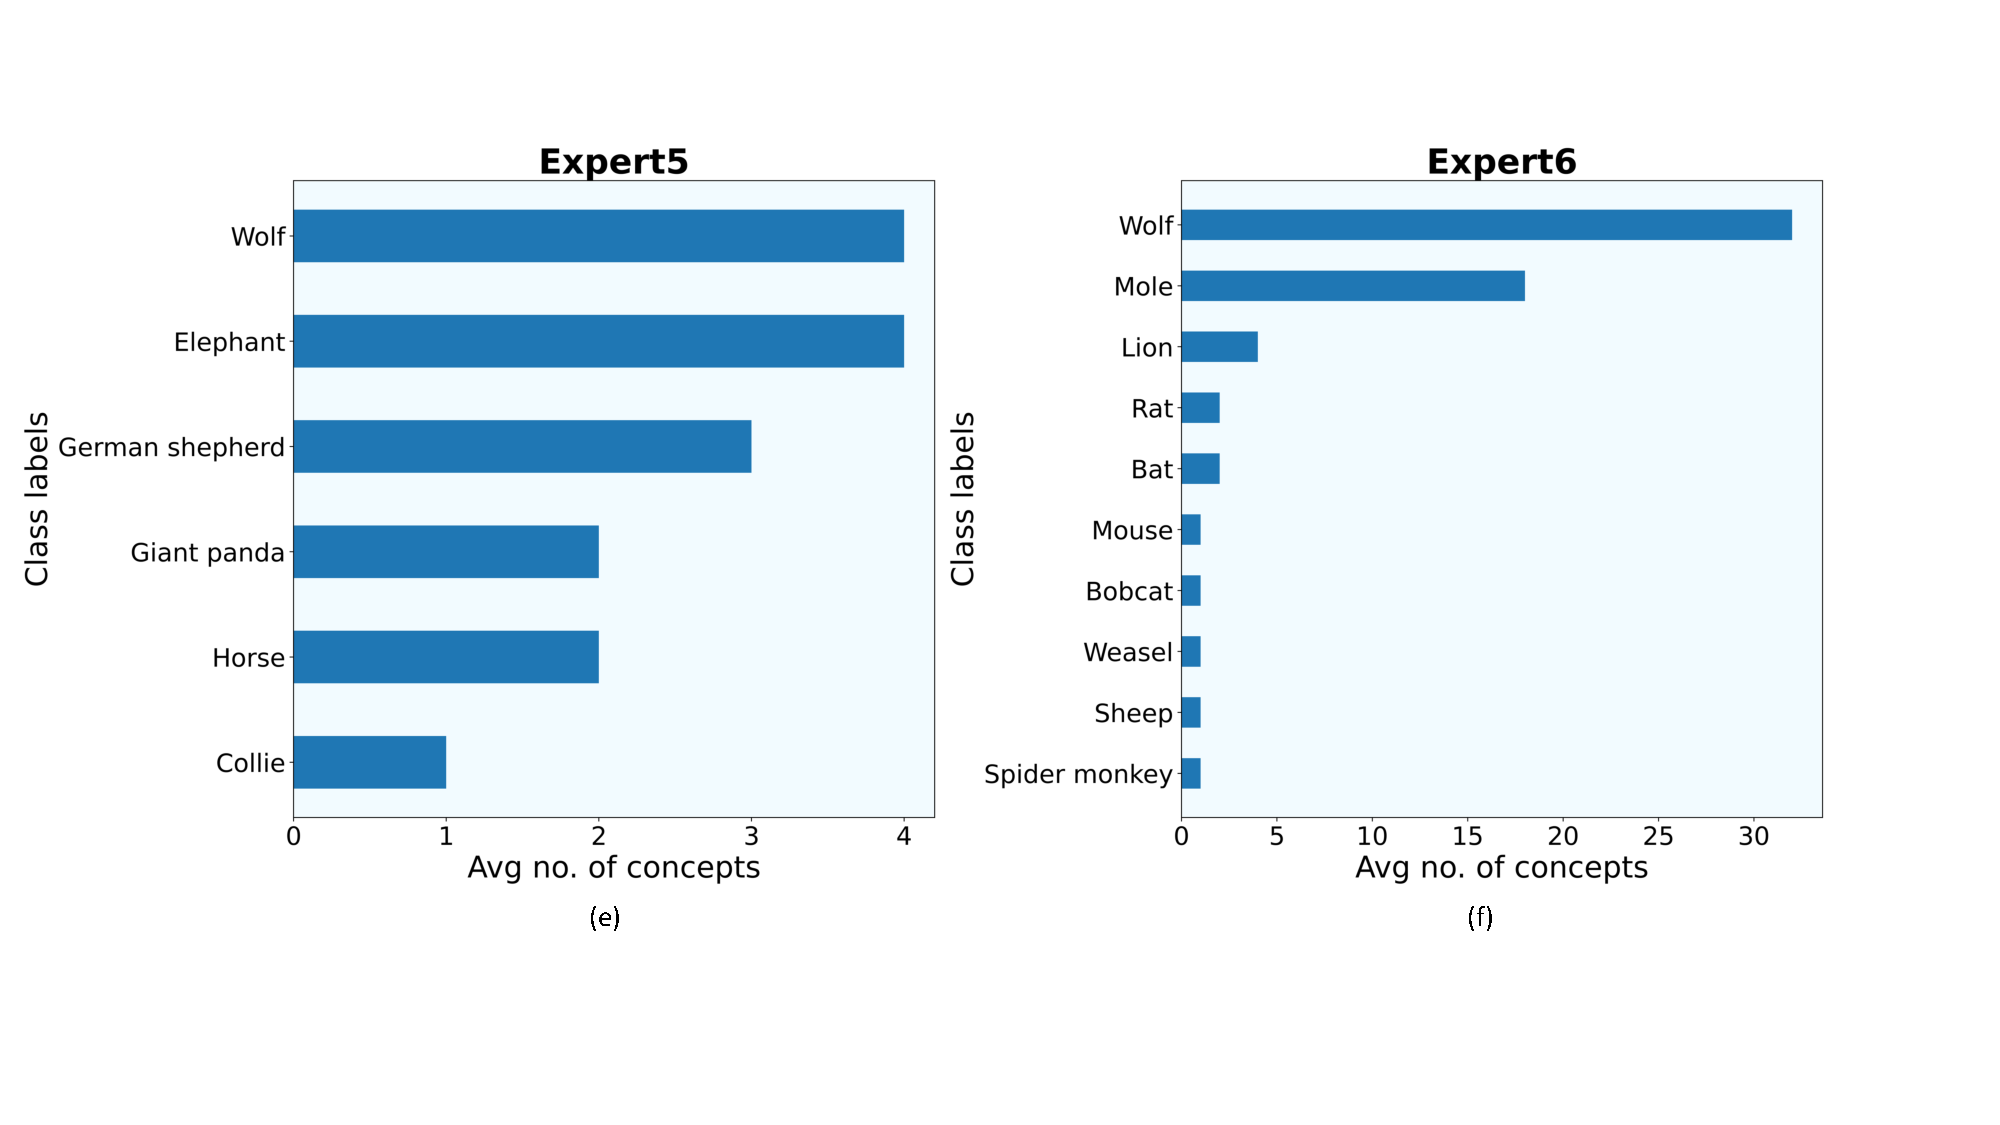
\includegraphics[width=1\textwidth]{figures/Supp/Avg_concept_class_VIT_Awa2_3.pdf} 
%   \label{fig:Awa2_VIT_c}} \\
%   \caption{Class labels (Animal species) vs avg concepts using VIT as backbone for Awa2. Each bar in this plot indicates the average number concepts required to explain each sample of that animal species correctly. \textcolor{red}{For example according to (a) expert1 requires approximately 80 concepts to explain an instance of ``Otter''}.} 
%   \label{fig:Awa2_VIT_concept}
% \end{figure}